\begin{filecontents*}{referencias.bib}
@standard{iso29148,
  author={{ISO/IEC/IEEE}},
  title={{ISO/IEC/IEEE 29148:2018}: Systems and software engineering --- Life cycle processes --- Requirements engineering},
  organization={International Organization for Standardization},
  year={2018},
  url={https://www.iso.org/standard/72089.html},
  note={Edici\'on 2, noviembre de 2018}
}
@standard{iso25010,
  author={{ISO/IEC}},
  title={{ISO/IEC 25010:2023}: Systems and software engineering --- Systems and software Quality Requirements and Evaluation (SQuaRE) --- Product quality model},
  organization={International Organization for Standardization},
  year={2023},
  url={https://www.iso.org/standard/78176.html}
}
@book{pohl2025,
  author={Klaus Pohl},
  title={Requirements Engineering: Fundamentals, Principles, and Techniques},
  edition={2},
  publisher={Springer},
  address={Berlin, Heidelberg},
  year={2025},
  isbn={978-3-662-69204-2},
  url={https://link.springer.com/book/9783662692042}
}
@book{swebok2024,
  editor={Hironori Washizaki},
  title={Guide to the Software Engineering Body of Knowledge (SWEBOK Guide), Version 4.0},
  publisher={IEEE Computer Society},
  year={2024},
  url={https://www.computer.org/education/bodies-of-knowledge/software-engineering}
}
@book{pmbok2021,
  author={{Project Management Institute}},
  title={A Guide to the Project Management Body of Knowledge (PMBOK Guide) and The Standard for Project Management},
  edition={7},
  publisher={Project Management Institute},
  year={2021},
  url={https://www.pmi.org/standards/pmbok}
}
@inproceedings{mavin2009,
  author={Alistair Mavin and Philip Wilkinson and Adrian Harwood and Mark Novak},
  title={Easy Approach to Requirements Syntax (EARS)},
  booktitle={2009 17th IEEE International Requirements Engineering Conference},
  pages={317--322},
  publisher={IEEE},
  year={2009},
  doi={10.1109/RE.2009.9}
}
@misc{lopdp2021,
  author={{Asamblea Nacional del Ecuador}},
  title={Ley Org\'anica de Protecci\'on de Datos Personales},
  howpublished={Registro Oficial, Quinto Suplemento n.\textordmasculine{} 459},
  year={2021},
  month=may,
  url={https://www.registroficial.gob.ec/quinto-suplemento-al-registro-oficial-no-459/}
}
\end{filecontents*}
\documentclass[11pt,a4paper]{article}
% Documento académico de equipo. Preparado para lectura, corrección y validación.
\usepackage[utf8]{inputenc}
\usepackage[T1]{fontenc}
\usepackage[spanish,es-tabla]{babel}
\usepackage[margin=2.3cm,headheight=18pt]{geometry}
\usepackage{lmodern}
\usepackage{graphicx}
\graphicspath{{figuras/}}
% Permite probar este archivo aunque todavía no se hayan añadido las figuras.
% Al crear la carpeta figuras/ y colocar los archivos originales, los inserta.
\newcommand{\imagensegura}[2][]{%
  \IfFileExists{figuras/#2}{\includegraphics[#1]{#2}}{%
    \fbox{\parbox[c][2.6cm][c]{0.85\linewidth}{\centering\footnotesize
    Figura pendiente de adjuntar:\\
    \texttt{\detokenize{#2}}}}%
  }%
}
\usepackage{array,booktabs,tabularx,longtable,multirow}
\usepackage{enumitem}
\usepackage[table]{xcolor}
\usepackage{fancyhdr,titlesec,float}
\usepackage{caption}
\usepackage{pdflscape}
\usepackage{hyperref}
\usepackage{cite}
\usepackage{microtype}
\usepackage{lastpage}

\hypersetup{colorlinks=true,urlcolor=blue,linkcolor=blue,citecolor=blue,pdftitle={MEDICLAB UTEQ - Fundamento, contexto y requisitos},pdfauthor={Equipo académico de Ingeniería de Requerimientos}}
\definecolor{azuluteq}{HTML}{123C61}
\definecolor{turquesa}{HTML}{008D92}
\definecolor{grisfondo}{HTML}{EEF6F7}
\fancyhf{}
\pagestyle{fancy}
\fancyhead[L]{\footnotesize UTEQ -- Ingeniería de Requerimientos}
\fancyhead[R]{\footnotesize PFC -- MEDICLAB UTEQ}
\fancyfoot[C]{\footnotesize \thepage\ / \pageref{LastPage}}
\setlength{\parindent}{0pt}
\setlength{\parskip}{4.7pt}
\setlength{\emergencystretch}{3em}
\setlist[itemize]{leftmargin=*,itemsep=2pt,topsep=2pt}
\setlist[enumerate]{leftmargin=*,itemsep=2pt,topsep=2pt}
\renewcommand{\arraystretch}{1.16}
\captionsetup{font=small,labelfont=bf}
\titleformat{\section}{\large\bfseries\color{azuluteq}}{\thesection.}{.65em}{}
\titleformat{\subsection}{\normalsize\bfseries\color{turquesa}}{\thesubsection.}{.6em}{}
\newcommand{\estado}[1]{\textbf{\textcolor{turquesa}{#1}}}
\newcommand{\fuenteimg}[1]{\textit{Fuente: captura propia del prototipo, anonimizada para divulgación académica. Archivo: \texttt{#1}.}}
\newcommand{\nota}[1]{\begin{quote}\small\textbf{Nota metodológica.} #1\end{quote}}
\begin{document}
\spanishplainpercent % evita error de glue al usar porcentajes en tablas
\hypersetup{pageanchor=false}
\begin{titlepage}
\centering
\vspace*{1.0cm}
{\Large\bfseries UNIVERSIDAD TÉCNICA ESTATAL DE QUEVEDO\par}
\vspace{0.25cm}
{\large FACULTAD DE CIENCIAS DE LA COMPUTACIÓN\par}
{\large CARRERA DE SOFTWARE\par}
\vspace{0.6cm}
\rule{\linewidth}{0.7mm}\\[0.2cm]
{\Huge\bfseries MEDICLAB UTEQ\par}
\vspace{0.2cm}
{\LARGE\bfseries Fundamentos, tipos de requisitos y contexto del sistema\par}
\vspace{0.25cm}
{\large\bfseries GA-PE-U · SUM · Práctica Experimental Unidad I\par}
\rule{\linewidth}{0.7mm}

\vspace{1.0cm}

\fcolorbox{turquesa}{grisfondo}{\parbox{0.88\linewidth}{\centering\vspace{0.3cm}
\textbf{Evidencia base:} 14 capturas originales de la interfaz MEDICLAB UTEQ.\\
\textbf{Estado académico:} análisis aplicado; perfiles interesados simulados, requisitos candidatos pendientes de validación.\\
\textbf{Enfoque:} ISO/IEC/IEEE 29148:2018, Pohl (2025), SWEBOK v4.0 y MoSCoW.
\vspace{0.3cm}}}

\vspace{1.0cm}

\begin{tabularx}{0.94\linewidth}{@{}lX@{}}
\textbf{Asignatura:} & Ingeniería de Requerimientos (ISR-401)\\
\textbf{Integrantes:}
 & ALVIA VILLEGAS ERICK ADALBERTO\\
 & CHALACÁN TOALÁ YERAI DAVID\\
\textbf{Docente:} & Gleiston Cicerón Guerrero Ulloa\\
\textbf{Modalidad:} & Grupal, estudio de sistema propio\\
\textbf{Fecha:} & Noviembre de 2026\\
\end{tabularx}
\vfill
{\small Quevedo -- Los Ríos -- Ecuador\\ 2026\par}
\end{titlepage}
\hypersetup{pageanchor=true}
\tableofcontents
\clearpage

% ==================== 00_organizacion ====================
\section{Sección 0. Identificación y organización del PFC}
\subsection{Conformación del equipo y responsabilidades}
El equipo está formado por 2 estudiantes. Para cubrir las cinco funciones indicadas en la Guia practica, se asignaran responsabilidades dobles cada que corresponda. La distribución constituye una \emph{propuesta de organización interna}: su aceptación definitiva fue acordada y posteriormente aceptada dentro de la coordinación del equipo.
\begin{table}[H]\centering\small
\caption{Distribución propuesta de funciones para tres integrantes.}\label{tab:roles}
\begin{tabularx}{\linewidth}{@{}p{4.4cm}p{3cm}X@{}}\toprule
\textbf{Integrante} & \textbf{Función principal} & \textbf{Función complementaria y tareas}\\\midrule
Chalacán Toalá Yerai David & Analista líder & Investigador C: integra las secciones 2.5--2.6; verifica cobertura de subtemas, citas y consistencia general.\\
Alvia Villegas Erick Adalberto & Investigador A/InvestigadorB & Documentador: desarrolla 2.1--2.4; organiza IEEE, portada, índice, tablas y fuentes LaTeX, verifica ejemplos y criterios de aceptación junto al analista líder..\\
\bottomrule
\end{tabularx}
\end{table}
La participación se debe acreditar mediante cambios identificables en el repositorio y/o revisión cruzada, sin atribuir entrevistas, pruebas o acuerdos no efectuados.
\subsection{Descripción del sistema (menos de 150 palabras)}
\textbf{MEDICLAB UTEQ} es un prototipo de sistema de gestion y información para apoyar las actividades administrativas y operativas de un laboratorio clínico. Sus interfaces se enfocara en mostrar la gestión de pacientes y médicos, áreas de laboratorio, exámenes y parámetros referenciales, además de órdenes médicas, consulta de resultados, administración de usuarios y generación de reportes. La solución busca reunir en una misma aplicación tareas que, al gestionarse de forma separada y manual, pueden ocasionar duplicación de registros, dificultades de consulta y errores de transcripción. Sus usuarios previstos incluyen personal de recepción, laboratorio, médicos, responsables de administración y supervisión del centro medico. La evidencia disponible corresponde a capturas de interfaz: estas permiten reconocer opciones de trabajo, pero cabe recalcar que no acredita la implementación, eficacia o seguridad de cada operación.
\subsection{Clasificación del tipo de sistema}
El PFC se considera principalmente un \textbf{sistema de información transaccional especializado en laboratorio clínico}, porque registra y consulta entidades operativas: pacientes, áreas, exámenes, órdenes y resultados. También presenta funciones de información gerencial mediante reportes. La interfaz tiene características de una aplicación de escritorio; no se puede deducir de las capturas el framework, el lenguaje de programación, el DBMS ni la topología de despliegue. Por ello, se descarta atribuirle una arquitectura cliente--servidor específica sin inspección del proyecto fuente. La tipología sigue las distinciones de sistemas y contexto de Pohl \cite{pohl2025}.
\subsection{Cinco stakeholders principales: perfiles simulados}
Los perfiles siguientes son \textbf{hipótesis de interesados}, no participantes reales ni sujetos entrevistados. Su poder e interés fueron estimados para practicar la matriz poder/interés de gestión de interesados; requieren validación con representantes del PFC \cite{pmbok2021}.
\begin{table}[H]\centering\scriptsize
\caption{Matriz preliminar de poder e interés.}\label{tab:stakeholders}
\begin{tabularx}{\linewidth}{@{}p{2.0cm}Xccp{2.8cm}@{}}\toprule
\textbf{Perfil} & \textbf{Necesidad hipotética} & \textbf{Poder} & \textbf{Interés} & \textbf{Estrategia sugerida}\\\midrule
Dirección del centro & Supervisar trazabilidad de órdenes, resultados e informes. & Alto & Alto & Gestionar de cerca.\\
Recepcionista & Registrar pacientes y localizar órdenes sin retrasos. & Bajo & Alto & Mantener informado y consultar.\\
Laboratorista & Administrar exámenes, parámetros y resultados sin errores. & Medio & Alto & Involucrar en validación funcional.\\
Médico solicitante & Asociar solicitudes a pacientes y consultar resultados autorizados. & Medio & Alto & Consultar escenarios y permisos.\\
Administrador TI & Controlar cuentas, roles, respaldos y operación. & Alto & Medio & Mantener satisfecho y coordinar riesgos.\\\bottomrule
\end{tabularx}
\end{table}
\textbf{Lectura de la matriz.} Dirección y administrador TI pueden influir sobre recursos y políticas; recepcionista y laboratorista aportan conocimiento del trabajo diario. La ubicación es una estimación metodológica, no un resultado de encuesta. El paciente es un beneficiario y titular de datos esencial, aunque para esta matriz inicial se haya priorizado a los cinco perfiles operativos solicitados.
\subsection{Base de evidencia y límites de inferencia}
\begin{table}[H]\centering\scriptsize
\caption{Lo observable frente a lo que todavía requiere comprobación.}\label{tab:evidencias}
\begin{tabularx}{\linewidth}{@{}p{3cm}Xp{3.8cm}@{}}\toprule
\textbf{Pantalla} & \textbf{Elemento visible} & \textbf{No demostrado solo con captura}\\\midrule
Pacientes & Filtros, tabla, botones Agregar/Editar/Eliminar y formulario de alta. & Validación de cédulas, persistencia o permisos.\\
Laboratorio y exámenes & Áreas, catálogo, parámetros, unidades y rangos. & Reglas clínicas o consistencia de rangos.\\
Órdenes médicas & Estados Borrador/Registrado; nuevo, editar, anular y resultados. & Transiciones permitidas y bitácora.\\
Resultados & Historial, consulta por filtros e impresión. & Exactitud, integridad y autorización.\\
Seguridad & Usuarios, roles y médicos con opciones de gestión. & Políticas de contraseñas y control de acceso efectivo.\\
Reportes & Vista previa de informe estructural con parámetros. & Auditoría, validación de cifras o exportación confiable.\\\bottomrule
\end{tabularx}
\end{table}
\nota{Las capturas originales contenían identificadores, teléfonos, correos y nombres. Las imágenes incluidas en este proyecto se anonimizaron antes de su incorporación; los originales no deben publicarse en GitHub.}


% ==================== 01_fundamento ====================

\section{Fundamento teórico aplicado al PFC}
\nota{La consigna asigna los apartados 2.1--2.6 entre investigadores, pero no proporciona sus títulos concretos. Se adopta aquí una estructura de seis subtemas coherentes con ISO/IEC/IEEE 29148:2018, Pohl (2025) y SWEBOK v4.0; el equipo debe compararla con el capítulo indicado por el docente. Las definiciones son síntesis y no citas textuales.}

\clearpage

\subsection{Necesidad, requisito y especificación (2.1)}
\textbf Un requisito representa una condición o capacidad que un sistema debe satisfacer para responder a una necesidad de una parte interesada. La especificación establece un registro organizado de dichas condiciones para orientar diseño, construcción y evaluación; ISO/IEC/IEEE 29148:2018 desarrolla los procesos y productos de ingeniería de requisitos \cite{iso29148}.

\textbfLa La diferencia principal radica en que la necesidad describe una dificultad directa del entorno y el requisito transforma esa preocupación en una obligación valida y comprobable. La frase "el laboratorio necesita ordenar mejor sus solicitudes" es verdad que puede guiar una conversación, pero todavía no explica qué datos deben conservarse especificamente. Una formulación como "el sistema deberá vincular cada orden a un paciente y a un médico seleccionado" restringe el resultado esperado y puede evaluarse con registros de prueba.

\textbf{Ejemplo.} La pantalla Nueva orden contiene campos para paciente, médico y examen, además de una lista de exámenes. Se deriva un candidato que prohíba guardar una orden sin estas asociaciones. No se afirma que la validación ya esté programada; debe probarse.

\subsection{Stakeholders, fuentes y elicitación (2.2)}
\textbf La elicitación reúne e interpreta necesidades de interesados a partir de personas, documentos, sistemas existentes y otras fuentes del dominio; la actividad debe complementarse con negociación y comprobación de lo obtenido \cite{pohl2025,swebok2024}.

\textbf Una captura de pantalla es evidencia de la existencia de controles, pero no evidencia de la motivación original de cada usuario. La persona de recepción puede priorizar búsquedas rápidas y por otro lado el técnico de laboratorio busca la exactitud de parámetros, por lo que sus expectativas podrían entrar en conflicto. La identificación de fuentes permite separar observaciones directas, hipótesis y decisiones, reduciendo el riesgo de convertir intuiciones en requisitos falsamente aprobados.

\textbf{Ejemplo.} En la vista Gestión de pacientes aparecen filtros por cédula, ciudad y teléfono. Una entrevista futura con un recepcionista podría verificar si la cédula es un identificador preferente, si la búsqueda debe aceptar coincidencias parciales y qué sucede ante registros duplicados. Por ahora, solo se confirma la presencia visual de esos filtros.

\subsection{Construcción y calidad de un requisito (2.3)}
\textbf ISO/IEC/IEEE 29148:2018 distingue la construcción de un requisito bien formado y las propiedades que permiten inspeccionarlo: necesidad, corrección, singularidad, ausencia de ambigüedad, verificabilidad y otras características relacionadas \cite{iso29148}. EARS proporciona patrones controlados de lenguaje natural, útiles para formular obligaciones sin imponer un diseño innecesario \cite{mavin2009}.

\textbf La redacción comienza identificando quién debe hacer qué y bajo cuál condición. Un requisito medible necesita un criterio que permita decidir si se cumplió, mientras que "el sistema será seguro" solo expresa un deseo general. La formulación debe describir el comportamiento observable y reservar decisiones de interfaz o tecnología cuando no estén justificadas por una restricción real.

\textbf{Ejemplo.} \emph{Ante el intento de guardar una orden sin médico asignado, MEDICLAB deberá rechazar la operación e informar el campo obligatorio ausente}. El evento y la respuesta son independientes de cómo se haya programado el formulario. La prueba consiste en dejar vacío el campo médico y observar si se conserva o no la orden.

\subsection{Tipos y niveles de requisitos (2.4)}
\textbf Las necesidades de negocio, las de las partes interesadas y las expectativas de los usuarios pueden conducir a requisitos del sistema y del software. Entre estos se distinguen comportamientos funcionales, propiedades de calidad, interfaces, desempeño, restricciones y condiciones de conformidad; las taxonomías son instrumentos de análisis, no categorías totalmente excluyentes \cite{iso29148,pohl2025}.

\textbf El requisito de negocio explica el valor perseguido, mientras que el funcional especifica el servicio necesario. Un requisito de calidad limita cómo debe comportarse una función, por ejemplo durante una búsqueda. Las restricciones, en cambio, delimitan decisiones permitidas, tales como políticas legales o condiciones de acceso, sin describir necesariamente una nueva función visible.

\textbf{Ejemplo.} Como objetivo de negocio se propone disminuir errores de asociación entre órdenes y pacientes; la función asociada obliga a guardar el identificador del paciente. El requisito de calidad exigiría que la consulta de una orden tarde como máximo tres segundos bajo una carga definida. La restricción legal exige tratamiento responsable de datos personales y de salud conforme a la regulación aplicable \cite{lopdp2021}.

\subsection{Contexto, límites y tipo de sistema (2.5)}
\textbf El contexto de ingeniería de requisitos reúne los objetos del entorno que afectan el sistema o reciben efectos de él. Distinguir límite del sistema, contexto relevante y alcance de desarrollo evita asignar a la solución responsabilidades de actores o servicios externos \cite{pohl2025}.

\textbf El laboratorio es una organización con procesos humanos; MEDICLAB es una herramienta dentro de ese proceso y no sustituye el juicio del profesional clínico. Aunque la pantalla contiene rangos de referencia, no existe evidencia para atribuirle la interpretación diagnóstica automática. La frontera debe revisarse cuando se identifiquen periféricos, sistemas hospitalarios o un DBMS real, ya que las imágenes no prueban esas integraciones.

\textbf{Ejemplo.} Se incluye la creación de pacientes y órdenes; se excluyen la toma física de muestras, las pruebas biológicas, los diagnósticos y la decisión clínica. La opción de impresión sugiere una relación con el servicio de impresión del equipo, pero su protocolo concreto permanece pendiente de análisis técnico.

\subsection{Validación, trazabilidad y gestión del cambio (2.6)}
\textbf La verificación examina si los artefactos cumplen condiciones especificadas; la validación comprueba si responden a las necesidades de los interesados. La trazabilidad enlaza necesidades, requisitos, diseños, pruebas y modificaciones, permitiendo evaluar el efecto de cambiar una decisión \cite{iso29148,swebok2024}.

\textbf Si se modifica la política de anulación de órdenes, puede cambiar el estado almacenado y el contenido de los reportes. Una matriz con identificadores permite localizar qué escenarios dependen de esa regla y qué pruebas deben repetirse. Por otro lado, una pantalla correcta visualmente no demuestra que los usuarios la acepten o que los datos se conserven sin errores; para ello hacen falta pruebas y revisión con interesados.

\textbf{Ejemplo.} Se establece un vínculo entre la necesidad de evitar órdenes incompletas, el requisito RF-06 y una prueba que intenta guardar sin examen seleccionado. La cadena se presenta como plan de validación, no como resultado de prueba ya realizada.

\subsection{Síntesis crítica de las seis nociones}
\begin{table}[H]\centering\small
\caption{Vinculación entre teoría y un artefacto comprobable del PFC.}
\begin{tabularx}{\linewidth}{@{}p{4.1cm}X@{}}\toprule
\textbf{Noción} & \textbf{Artefacto del informe / cuestión que responde}\\\midrule
Necesidad y requisito & Catálogo de requisitos: ¿qué resultado debe existir?\\
Elicitación & Matriz de perfiles y preguntas: ¿quién necesita ese resultado?\\
Formulación & Estructura EARS y criterios: ¿es comprobable?\\
Clasificación & Tabla de tipos, prioridad y fuentes: ¿qué nivel y naturaleza tiene?\\
Contexto & Diagrama de frontera y entidades: ¿qué queda dentro y fuera?\\
Validación / cambio & Matriz de trazabilidad y pruebas: ¿cómo se comprobará y actualizará?\\\bottomrule
\end{tabularx}
\end{table}


% ==================== 02_requisitos ====================

\section{Tabla de tipos de requisitos aplicados a MEDICLAB}
\subsection{Convenciones de redacción y priorización}
Se establecen identificadores persistentes con prefijos \texttt{BN} (negocio), \texttt{ST} (stakeholder), \texttt{US} (usuario), \texttt{RF} (funcional), \texttt{IF} (interfaz), \texttt{RD} (rendimiento), \texttt{NQ} (calidad), \texttt{CT} (restricción) y \texttt{CP} (conformidad). La forma «\emph{cuando} ocurre [evento], MEDICLAB \emph{deberá} [respuesta]» se inspira en la redacción controlada EARS \cite{mavin2009} y en las propiedades de requisitos de ISO/IEC/IEEE 29148:2018 \cite{iso29148}. Las prioridades MoSCoW son asignaciones preliminares del equipo y \textbf{no representan un acuerdo con stakeholders reales}.

\begin{table}[H]\centering\small
\caption{Criterio utilizado para la priorización MoSCoW.}\label{tab:moscow}
\begin{tabularx}{\linewidth}{@{}p{2.5cm}X@{}}\toprule
\textbf{Nivel} & \textbf{Interpretación en esta iteración académica}\\\midrule
Must & Indispensable para operaciones centrales o para proteger datos personales.\\
Should & Necesario para operar con calidad, aunque puede tener solución transitoria.\\
Could & Mejora de valor que no impide demostrar el flujo principal.\\
Won't (ahora) & Fuera del alcance de esta versión y no recogido como compromiso de construcción.\\\bottomrule
\end{tabularx}
\end{table}

\subsection{Catálogo de veinte requisitos candidatos}
\begingroup\footnotesize\setlength{\tabcolsep}{3.5pt}
\begin{longtable}{|p{1.3cm}|p{2.35cm}|p{7.3cm}|p{2.4cm}|}
\caption{Veinte requisitos del PFC: redacción, tipo, prioridad y fuente.}\label{tab:catalogo}\\\hline
\textbf{ID} & \textbf{Tipo / MoSCoW} & \textbf{Enunciado de requisito candidato} & \textbf{Origen observable o supuesto}\\\hline\endfirsthead
\hline\textbf{ID} & \textbf{Tipo / MoSCoW} & \textbf{Enunciado (continuación)} & \textbf{Fuente}\\\hline\endhead
\textbf{BN-01} & Negocio / Must & El centro deberá disponer de un registro único para identificar las órdenes de exámenes asociadas a los pacientes en el proceso interno. & Necesidad inferida del módulo Órdenes; S1.\\\hline
\textbf{ST-01} & Stakeholder / Must & El responsable simulado del laboratorio deberá poder consultar la cantidad de órdenes registradas y sus estados por período de búsqueda. & Perfil simulado S1; vista Órdenes.\\\hline
\textbf{US-01} & Usuario / Should & El recepcionista deberá poder localizar a un paciente mediante el campo de cédula antes de iniciar su registro en una nueva orden. & Vista Pacientes; S2.\\\hline
\textbf{RF-01} & Funcional / Must & Cuando el operador complete los campos obligatorios de alta, MEDICLAB deberá registrar el paciente y asignarle un identificador interno. & Modal Nuevo paciente.\\\hline
\textbf{RF-02} & Funcional / Must & Cuando se indique una cédula existente en el filtro, MEDICLAB deberá presentar el registro de paciente que coincida con ese valor. & Vista Pacientes.\\\hline
\textbf{RF-03} & Funcional / Should & Cuando un administrador de laboratorio confirme el nombre de una nueva área, MEDICLAB deberá agregarla al catálogo de áreas. & Modal Nueva área.\\\hline
\textbf{RF-04} & Funcional / Must & Cuando se cree un examen, MEDICLAB deberá asociar su nombre con una de las áreas de laboratorio registradas. & Modal Nuevo examen.\\\hline
\textbf{RF-05} & Funcional / Must & Cuando el laboratorista guarde un parámetro, MEDICLAB deberá asociar su descripción, unidad y rango referencial al examen elegido. & Configuración parámetros.\\\hline
\textbf{RF-06} & Funcional / Must & Cuando se confirme una nueva orden con paciente, médico y al menos un examen seleccionados, MEDICLAB deberá crear la orden y generar su identificador. & Modal Nueva orden.\\\hline
\textbf{RF-07} & Funcional / Should & Cuando un usuario autorizado anule una orden seleccionada, MEDICLAB deberá cambiar su estado a Anulada y excluirla de órdenes vigentes. & Acción Anular orden; regla propuesta.\\\hline
\textbf{RF-08} & Funcional / Should & Cuando se filtre el historial por cédula o paciente, MEDICLAB deberá listar solo los resultados relacionados con el criterio de búsqueda. & Vista Historial resultados.\\\hline
\textbf{RF-09} & Funcional / Should & Cuando el operador seleccione el reporte estructural de exámenes, MEDICLAB deberá mostrar área, examen, parámetro, unidad y rango almacenados. & Vista Reporte estructural.\\\hline
\textbf{IF-01} & Interfaz / Should & Cuando el usuario solicite imprimir el reporte visible, MEDICLAB deberá transferir una representación imprimible al subsistema de impresión configurado. & Icono de impresión; verificar interfaz.\\\hline
\textbf{RD-01} & Rendimiento / Should & La búsqueda exacta de un paciente deberá responder en un percentil 95 de 3 segundos o menos, con 10 usuarios concurrentes y 10\,000 registros de prueba. & Objetivo propuesto, no medido.\\\hline
\textbf{NQ-01} & Calidad / Must & MEDICLAB deberá denegar el acceso a resultados de pacientes a cuentas sin el permiso de consulta de resultados. & Riesgo de confidencialidad; S5.\\\hline
\textbf{NQ-02} & Calidad / Must & MEDICLAB deberá rechazar la creación de órdenes cuya referencia a paciente, médico o examen no corresponda a un registro existente. & Integridad referencial propuesta.\\\hline
\textbf{NQ-03} & Calidad / Should & El formulario Nueva orden deberá permitir que 9 de 10 usuarios de prueba completen la creación en 3 minutos o menos, sin ayuda. & Objetivo de operabilidad supuesto.\\\hline
\textbf{NQ-04} & Calidad / Should & MEDICLAB deberá mantener accesible la consulta de órdenes durante al menos el 99\,\% de los minutos de una ventana de prueba de 30 días. & Objetivo de disponibilidad supuesto.\\\hline
\textbf{CT-01} & Restricción / Must & MEDICLAB no deberá asociar un examen a una orden si el examen no pertenece al catálogo vigente de la organización. & Regla de dominio propuesta.\\\hline
\textbf{CP-01} & Conformidad / Must & El responsable del sistema deberá disponer de un procedimiento documentado y aprobado para controlar acceso y tratamiento de datos de pacientes antes del uso con información real. & LOPDP, exigencia de proceso por validar.\\\hline
\end{longtable}\endgroup

\subsection{Clasificación de los cinco requisitos de calidad}
\begin{table}[H]\centering\small
\caption{ISO/IEC 25010:2023, métrica, unidad y criterio verificable propuesto.}\label{tab:calidad}
\begin{tabularx}{\linewidth}{@{}p{1.2cm}p{3.1cm}Xp{3.5cm}@{}}\toprule
\textbf{ID} & \textbf{Característica / subcaracterística} & \textbf{Métrica y condiciones} & \textbf{Aceptación propuesta}\\\midrule
RD-01 & Eficiencia de desempeño / comportamiento temporal & Percentil 95 del tiempo entre Buscar y aparición de resultados con 10 usuarios simultáneos y 10\,000 pacientes ficticios. & $P_{95}\leq3$ segundos sobre 200 consultas.\\
NQ-01 & Seguridad / confidencialidad & Proporción de lecturas no autorizadas bloqueadas entre perfiles simulados. & 30 de 30 intentos rechazados; 0 resultados expuestos.\\
NQ-02 & Seguridad / integridad & Número de órdenes con claves de relación inválidas después del ensayo. & 0 órdenes huérfanas en 100 intentos de alta.\\
NQ-03 & Capacidad de interacción / operabilidad & Tasa de éxito y tiempo de completar Nueva orden con usuarios evaluadores. & $\geq90\,\%$ de 10 personas, $\leq3$ min, sin ayuda.\\
NQ-04 & Fiabilidad / disponibilidad & Porcentaje de minutos en que funciona Consulta de órdenes en 30 días. & Disponibilidad $\geq99\,\%$; medición cada minuto.\\\bottomrule
\end{tabularx}
\end{table}
Las características se alinean con el modelo de calidad de producto de ISO/IEC 25010:2023 \cite{iso25010}. En un prototipo académico el tamaño de carga y los umbrales solo sirven para definir pruebas futuras: es incorrecto interpretarlos como niveles alcanzados.

\subsection{Criterios de aceptación y pruebas propuestas}
\begingroup\footnotesize
\begin{longtable}{|p{1.4cm}|p{5.4cm}|p{7.0cm}|}
\caption{Plan de verificación del catálogo. No se afirma ejecución.}\label{tab:pruebas}\\\hline
\textbf{ID} & \textbf{Escenario de prueba} & \textbf{Resultado que permitiría aceptar el requisito}\\\hline\endfirsthead\hline\textbf{ID} & \textbf{Escenario} & \textbf{Resultado esperado}\\\hline\endhead
BN-01 & Registrar 5 órdenes de ejemplo para 2 pacientes. & Cada orden posee ID único y vínculo a un paciente.\\\hline
ST-01 & Consultar el período que contiene las cinco órdenes. & Los conteos por estado coinciden con la muestra.\\\hline
US-01 & Buscar cédula ficticia antes de crear orden. & El registro correcto se puede identificar en la consulta.\\\hline
RF-01 & Guardar formulario válido de paciente ficticio. & Alta visible con identificador diferente a otros registros.\\\hline
RF-02 & Buscar por cédula exacta conocida. & Se obtiene solo el paciente coincidente.\\\hline
RF-03 & Agregar un área «Serología de prueba». & Nueva área disponible en la lista.\\\hline
RF-04 & Crear examen en un área existente. & El examen mantiene el área elegida al consultar.\\\hline
RF-05 & Registrar parámetro con nombre/unidad/rango ficticios. & La ficha del examen muestra la relación completa.\\\hline
RF-06 & Guardar una orden con paciente, médico y examen válidos. & Una orden nueva aparece con ID y sus vínculos.\\\hline
RF-07 & Anular orden de prueba y recargar consulta. & Estado Anulada visible; no aparece como vigente.\\\hline
RF-08 & Filtrar por paciente con 2 resultados conocidos. & Se muestran las 2 coincidencias y ninguna ajena.\\\hline
RF-09 & Generar reporte de un área configurada. & Coinciden área, examen, parámetros y unidades.\\\hline
IF-01 & Seleccionar imprimir desde el visor de reporte. & El subsistema abre una vista/cola imprimible correcta.\\\hline
RD-01 & Ejecutar 200 consultas con 10 sesiones simultáneas. & Al menos 95\,\% en 3 segundos o menos.\\\hline
NQ-01 & Intentar abrir resultados desde rol sin permiso. & Los 30 intentos fallan sin revelar contenido.\\\hline
NQ-02 & Enviar 100 altas con referencias inexistentes. & No queda ninguna orden guardada con referencia inválida.\\\hline
NQ-03 & Observar 10 participantes en la tarea Nueva orden. & Al menos 9 completan en 3 min sin ayuda.\\\hline
NQ-04 & Monitorizar cada minuto por 30 días. & Se alcanza como mínimo 99\,\% de disponibilidad.\\\hline
CT-01 & Intentar asignar un examen eliminado o desconocido. & El sistema bloquea la asociación.\\\hline
CP-01 & Inspeccionar política, responsables y registros de aprobación. & Existe documento aprobado antes de datos reales.\\\hline
\end{longtable}\endgroup

\subsection{Análisis de defectos y refinamiento de redacción}
\begin{table}[H]\centering\small
\caption{Comparación entre formulaciones iniciales y resultados revisables.}\label{tab:defectos}
\begin{tabularx}{\linewidth}{@{}p{2cm}Xp{5.5cm}@{}}\toprule
\textbf{Caso} & \textbf{Defecto de la formulación inicial} & \textbf{Reformulación}\\\midrule
«Sistema rápido» & No indica operación, usuarios, tamaño de datos ni umbral. & RD-01 fija consulta, volumen, concurrentes y $P_{95}$.\\
«Usuarios seguros» & Confunde seguridad con una percepción no medible. & NQ-01 define quién no accede y pruebas de denegación.\\
«Orden correcta» & No permite demostrar integridad del registro. & RF-06 y NQ-02 separan creación de integridad.\\
«Reportes inmediatos» & El término temporal carece de magnitud. & RF-09 define campos; medición de rapidez sería otro requisito.\\
«Todos los pacientes» & Universal impreciso sin considerar permisos y datos de prueba. & US-01 delimita búsqueda de un paciente por criterio.\\\bottomrule
\end{tabularx}
\end{table}

\subsection{Matriz de trazabilidad preliminar}
\begingroup\small
\begin{longtable}{@{}p{1.5cm}p{3.2cm}p{4.2cm}p{3.5cm}@{}}
\caption{Relaciones iniciales entre origen, requisito y evidencia esperada.}\label{tab:traza}\\\toprule
\textbf{ID} & \textbf{Fuente} & \textbf{Requisito relacionado} & \textbf{Verificación futura}\\\midrule\endfirsthead\toprule\textbf{ID} & \textbf{Fuente} & \textbf{Relación} & \textbf{Verificación}\\\midrule\endhead
BN-01 & Pantalla Órdenes & RF-06, NQ-02 & Órdenes con IDs y vínculos\\
ST-01 & Perfil Dirección (supuesto) & RF-09 & Reportes / conteo\\
US-01 & Pantalla Pacientes & RF-02 & Búsqueda exacta\\
RF-01--02 & Pacientes / nuevo paciente & RD-01, NQ-01 & Alta y filtrado\\
RF-03--05 & Área / examen / parámetros & CT-01 & Relación catálogos\\
RF-06--07 & Nueva orden y Órdenes & NQ-02 & Alta y anulación\\
RF-08--09 & Resultados / reportes & NQ-01, IF-01 & Filtrado y presentación\\
IF-01 & Visor del reporte & RF-09 & Impresión de prueba\\
RD-01 & Meta de calidad propuesta & RF-02 & Prueba de carga\\
NQ-01--04 & Riesgos / objetivos propuestos & RF-01, RF-06, RF-08 & Seguridad, carga y usabilidad\\
CT-01 & Dominio de exámenes (supuesto) & RF-04, RF-06 & Asociación inválida\\
CP-01 & Ley ecuatoriana & NQ-01 & Evaluación de cumplimiento\\\bottomrule
\end{longtable}\endgroup

La matriz aporta trazabilidad conceptual, pero no prueba que las funcionalidades funcionen. Para una línea base real deben añadirse el propietario del requisito, versión, fecha de aprobación, registro del stakeholder que lo valida y el resultado de ejecución de casos de prueba.


% ==================== 03_contexto ====================
\clearpage
\section{Límite del sistema, visión y contexto}
\subsection{Límite funcional del PFC}
El sistema de interés es la \textbf{aplicación MEDICLAB UTEQ} y su comportamiento de registro, consulta y presentación de información. Dentro del límite se consideran las pantallas y reglas propuestas para pacientes, médicos, áreas, exámenes, parámetros, órdenes, resultados, roles y reportes. Fuera del límite permanecen la atención clínica, la extracción y análisis físico de muestras, la interpretación diagnóstica, la emisión de documentos clínicos firmados por profesionales y la infraestructura no evidenciada por las imágenes.

\textbf{Restricción importante.} La interfaz muestra un botón de impresión y un visor de reportes, pero ello no demuestra que MEDICLAB pueda intercambiar datos con hospitales, aseguradoras, sistemas contables o instrumentos de laboratorio. Estos componentes no se incorporan como integraciones ya existentes. La frontera y el alcance se describen siguiendo la noción de contexto y límite de sistema de Pohl \cite{pohl2025}.

\begin{figure}[H]\centering
\IfFileExists{}{
    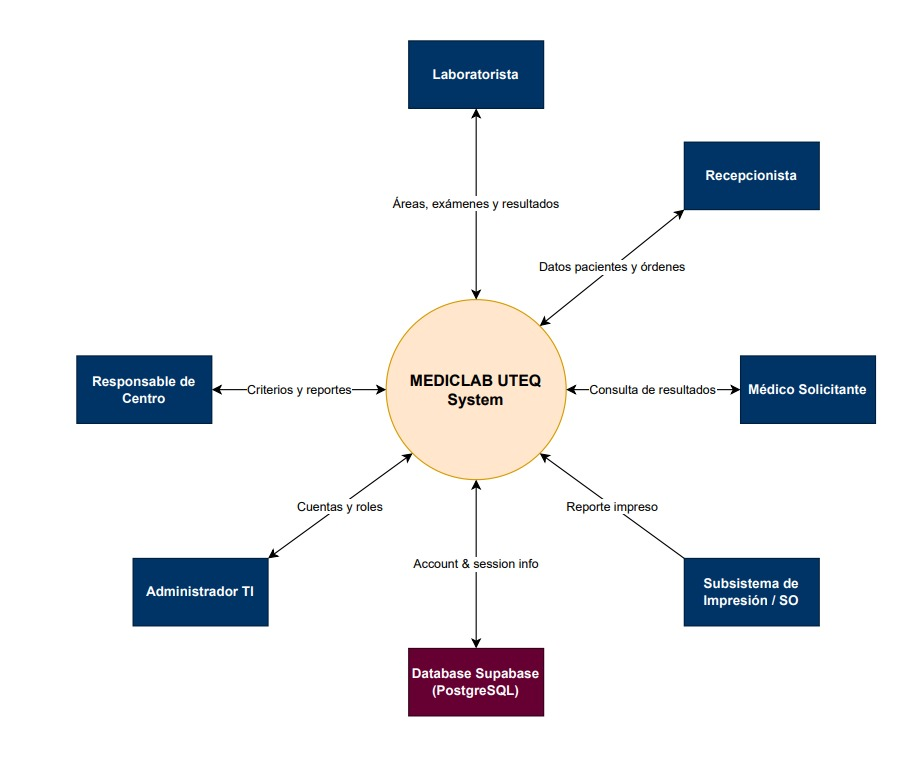
\includegraphics[
        width=15.80\linewidth,
        height=12.0cm,
        keepaspectratio
    ]{Figuras/DiagramaContextual.jpeg}
}{
    \fbox{
        \parbox[c][6.5cm][c]{.72\linewidth}{
            \centering 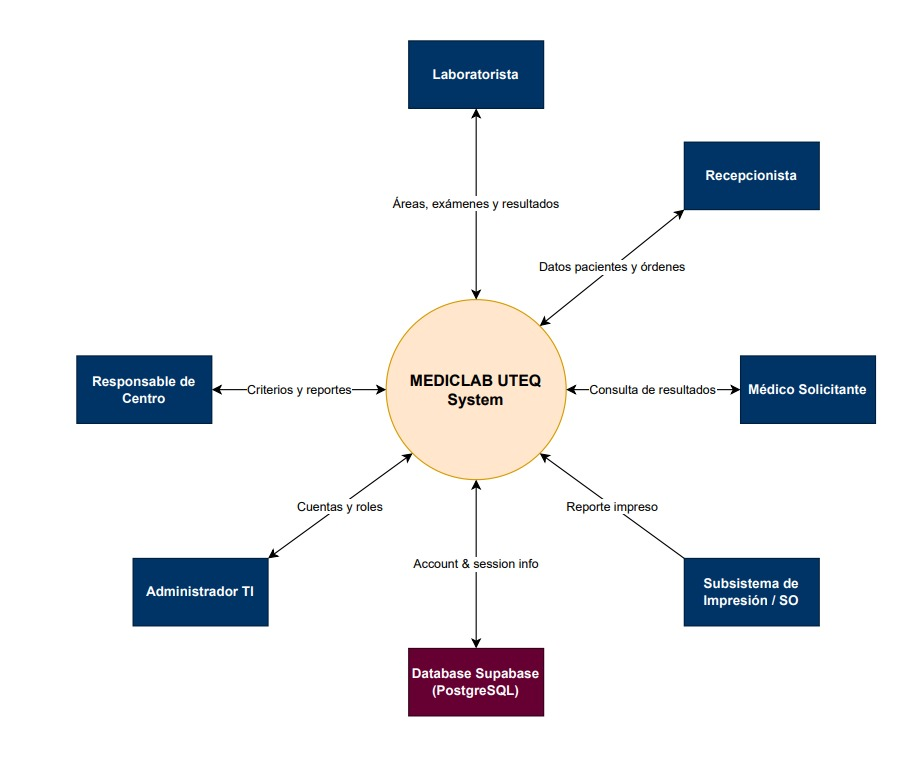
\includegraphics[width=4.95\linewidth, height=6.2cm, keepaspectratio]{Figuras/DiagramaContextual.jpeg}        
        }
    }
}
\vspace{1.0cm}
\caption{Diagrama preliminar de contexto y entidades externas. La línea de impresión es una interfaz por validar.}\label{fig:contexto}
\end{figure}


La Figura~\ref{fig:contexto} representa a cinco perfiles humanos y un posible servicio de impresión. Las personas aparecen como entidades externas al software, aun cuando actúen sobre la interfaz. Se utiliza un modelo de frontera funcional, no una arquitectura física de componentes.

\subsection{Entidades externas, intercambios y frecuencia}
\begin{table}[H]\centering\scriptsize
\caption{Interfaces de contexto: protocolo y frecuencia sin inventar integraciones.}\label{tab:interfaces}
\begin{tabularx}{\linewidth}{@{}p{2.4cm}p{2.5cm}Xp{2.7cm}p{1.7cm}@{}}\toprule
\textbf{Entidad externa} & \textbf{Tipo} & \textbf{Datos intercambiados} & \textbf{Interfaz / protocolo} & \textbf{Frecuencia}\\\midrule
Recepcionista & Persona & Identificación y datos de contacto de pacientes; filtros de búsqueda; órdenes. & Interfaz gráfica de aplicación. & A demanda.\\
Laboratorista & Persona & Áreas, exámenes, parámetros, unidades y resultados. & Interfaz gráfica de aplicación. & A demanda.\\
Médico solicitante & Persona & Selección de médico en orden; necesidades de consulta de resultados. & Interfaz gráfica; acceso propio por confirmar. & Por solicitud.\\
Administrador TI & Persona & Cuentas, roles y datos de médicos. & Interfaz de gestión de usuarios. & Eventual.\\
Responsable del centro & Persona & Consultas, criterios de reporte y vistas de informes. & Interfaz de reportes. & Periódica / a demanda.\\
Impresora / visor del SO & Subsistema externo hipotético & Documento imprimible de resultados o reportes. & Servicio de impresión del SO, por verificar. & Por solicitud.\\\bottomrule
\end{tabularx}
\end{table}
\textbf{Interpretación de la columna de frecuencia:} «a demanda», «eventual» y «periódica» describen patrones esperados de uso, no frecuencias medidas. Los valores exactos (eventos/día) y protocolos técnicos (IP, TLS, ODBC, etc.) se documentarán después de inspeccionar la arquitectura y los registros del prototipo.

\subsection{Visión del producto en formato Moore}
\begin{quote}
\small\textit{Para} el personal de recepción, laboratorio y administración de un centro de análisis clínicos \textit{que necesita} registrar pacientes y organizar exámenes, órdenes, resultados y reportes, \textit{MEDICLAB UTEQ es} una aplicación de información operativa \textit{que ofrece} consulta y mantenimiento de datos en módulos relacionados. \textit{A diferencia de} trabajar con registros separados y búsquedas manuales, \textit{nuestro producto} propone reunir la información de pacientes, catálogos y órdenes en una misma herramienta, con controles de acceso e integridad que aún deben validarse.
\end{quote}
La visión distingue población objetivo, necesidad, categoría, beneficio, alternativa y diferenciación. Evita afirmar beneficios cuantitativos (reducción de errores o tiempos) que todavía no han sido medidos en un estudio comparativo.

\subsection{Alcance actual y evolución propuesta}
\begin{table}[H]\centering\small
\caption{Control preliminar de alcance frente a expectativas futuras.}\label{tab:alcance}
\begin{tabularx}{\linewidth}{@{}p{3cm}X@{}}\toprule
\textbf{Grupo} & \textbf{Delimitación}\\\midrule
Visible en prototipo & Formularios y listados de pacientes, áreas, exámenes, órdenes, resultados, seguridad de usuarios/médicos y reportes.\\
Propuesto para validar & Reglas de integridad, seguridad de roles, automatización de pruebas, umbrales de rendimiento y disponibilidad.\\
Fuera del PFC actual & Diagnóstico médico automatizado, laboratorio físico, historia clínica completa, facturación electrónica, telemedicina e integraciones no demostradas.\\
Datos reservados & Identificaciones, correos y teléfonos de pacientes/usuarios presentes en capturas originales. No se publican.\\\bottomrule
\end{tabularx}
\end{table}

\subsection{Riesgos y supuestos asociados al límite}
\begin{enumerate}
\item \textbf{Uso clínico sin validación.} Las unidades y rangos mostrados son datos del prototipo y no deben usarse para decisiones médicas hasta su revisión profesional.
\item \textbf{Fuga de información.} El sistema contiene datos identificativos y potencialmente sensibles; el tratamiento necesita controles y base jurídica pertinente \cite{lopdp2021}.
\item \textbf{Reglas incompletas.} No se han visto pruebas de la transición entre Borrador, Registrado y Anulado; se requiere modelar y probar ese ciclo de vida.
\item \textbf{Dependencia de infraestructura.} No se conoce la tecnología de persistencia ni el procedimiento de respaldo; las propuestas de disponibilidad y recuperabilidad son pendientes.
\item \textbf{Actores no observados.} Que una orden tenga un médico asociado no demuestra que exista un portal propio para el médico; el acceso real debe verificarse.
\end{enumerate}


% ==================== 04_perspectivas ====================

\section{Ocho perspectivas de contexto aplicadas a MEDICLAB}
Las ocho perspectivas se toman de la estructura del capítulo 15 de Pohl (2025): \emph{uso, dominio, sistemas de TI, desarrollo, negocio, innovación, sociedad y técnica} \cite{pohl2025}. Cada perspectiva propone tres preguntas de elicitación y dos candidatos adicionales de requisito o restricción. \textbf{Estos dieciséis candidatos de descubrimiento} no se incorporan automáticamente a los veinte requisitos de la tabla~\ref{tab:catalogo}: representan decisiones aún pendientes y requieren acuerdo con interesados.

\subsection{Perspectiva de uso (Usage perspective)}
La evidencia de ventanas de búsqueda, formularios y menús permite examinar secuencias reales de trabajo, pero no su duración ni su comodidad.
\textbf{Preguntas de elicitación:}
\begin{enumerate}[label=\alph*)]
\item ¿En qué momento el recepcionista comprueba que un paciente está registrado antes de crear una orden?
\item ¿Qué datos debe poder completar el laboratorista durante una sesión de ingreso de resultados?
\item ¿Qué errores ocurren cuando el usuario vuelve de una pantalla a otra sin guardar?
\end{enumerate}
\textbf{Candidatos emergentes:}
\begin{itemize}
\item \textbf{P-USO-01 (funcional):} al seleccionar un paciente en una búsqueda, MEDICLAB deberá conservar su identificador al abrir el formulario Nueva orden.
\item \textbf{P-USO-02 (calidad):} el sistema deberá informar de los campos obligatorios ausentes en un formulario antes de autorizar su guardado.
\end{itemize}
\textbf{Conexión con el catálogo:} US-01 y RF-06. Los candidatos requieren pruebas con datos ficticios.

\subsection{Perspectiva del dominio (Subject perspective)}
La organización de exámenes por áreas y parámetros es específica del laboratorio. La semántica de las entidades debe acordarse con responsables del dominio, no deducirse únicamente de las etiquetas.
\textbf{Preguntas de elicitación:}
\begin{enumerate}[label=\alph*)]
\item ¿Una misma prueba puede asociarse a varias áreas o solo a una?
\item ¿Quién autoriza la modificación de rangos referenciales de un examen?
\item ¿Cuál es el ciclo de vida permitido entre Borrador, Registrado, Atendido y Anulado?
\end{enumerate}
\textbf{Candidatos emergentes:}
\begin{itemize}
\item \textbf{P-DOM-01 (restricción):} ninguna orden podrá asociar un examen desactivado en el catálogo vigente.
\item \textbf{P-DOM-02 (funcional):} toda modificación a un parámetro referencial deberá conservar su valor anterior, el usuario responsable y la fecha del cambio.
\end{itemize}
\textbf{Conexión:} RF-04, RF-05, CT-01 y un requisito futuro de auditoría. Las reglas clínicas precisas son desconocidas.

\subsection{Perspectiva de sistemas de TI (IT system perspective)}
Esta perspectiva considera sistemas informáticos existentes o externos que pueden condicionar el nuevo sistema. Las imágenes solo permiten confirmar pantallas, no servicios de red, bases de datos ni protocolos particulares.
\textbf{Preguntas de elicitación:}
\begin{enumerate}[label=\alph*)]
\item ¿Qué mecanismo de persistencia utiliza la aplicación y cómo se realizan respaldos?
\item ¿El visor de reportes entrega datos a un motor de impresión o solamente genera una vista previa?
\item ¿Existen interfaces aprobadas con un sistema hospitalario o de facturación?
\end{enumerate}
\textbf{Candidatos emergentes:}
\begin{itemize}
\item \textbf{P-TI-01 (interfaz):} la salida de un reporte estructural deberá conservar las mismas columnas y valores que la vista previa mostrada.
\item \textbf{P-TI-02 (restricción):} no se incluirá integración con terceros sin documentar contrato, autorización y formato de intercambio.
\end{itemize}
\textbf{Conexión:} IF-01, RF-09. El protocolo exacto permanece abierto.

\subsection{Perspectiva de desarrollo (Development perspective)}
Abarca recursos y decisiones del equipo que pueden limitar la especificación. Al no haberse inspeccionado el repositorio, no se atribuye un lenguaje o framework particular al prototipo.
\textbf{Preguntas de elicitación:}
\begin{enumerate}[label=\alph*)]
\item ¿Qué tecnologías y versiones se encuentran realmente en el repositorio del proyecto?
\item ¿Quién revisa los cambios sobre pacientes, órdenes y permisos antes de integrar código?
\item ¿Cómo se preparan datos ficticios reproducibles para las pruebas de aceptación?
\end{enumerate}
\textbf{Candidatos emergentes:}
\begin{itemize}
\item \textbf{P-DES-01 (proceso):} cada cambio de comportamiento de una orden deberá incluir al menos un caso de prueba revisado.
\item \textbf{P-DES-02 (restricción):} los entornos públicos de pruebas deberán emplear exclusivamente datos ficticios o anonimizados.
\end{itemize}
\textbf{Conexión:} CP-01 y mantenimiento de trazabilidad del informe.

\subsection{Perspectiva de negocio (Business perspective)}
Se examinan beneficios y políticas organizativas sin atribuir cifras ficticias de reducción de costos, errores o tiempos.
\textbf{Preguntas de elicitación:}
\begin{enumerate}[label=\alph*)]
\item ¿Qué problema operativo tiene mayor costo: duplicaciones, demoras o inconsistencias de resultados?
\item ¿Qué informes necesita la dirección para tomar decisiones administrativas?
\item ¿Qué procedimiento debe seguir una orden anulada para conservar responsabilidad y rastreo?
\end{enumerate}
\textbf{Candidatos emergentes:}
\begin{itemize}
\item \textbf{P-NEG-01 (negocio):} el centro deberá poder identificar las órdenes que cambiaron de estado durante un período seleccionado.
\item \textbf{P-NEG-02 (funcional):} el informe mensual deberá presentar el número de órdenes por estado y por período de consulta.
\end{itemize}
\textbf{Conexión:} BN-01, ST-01, RF-07. El valor económico debe comprobarse antes de prometer beneficios.

\subsection{Perspectiva de innovación (Innovation perspective)}
Permite proponer funciones nuevas diferenciando el prototipo actual de una evolución posible. La creatividad no demuestra automáticamente viabilidad ni necesidad.
\textbf{Preguntas de elicitación:}
\begin{enumerate}[label=\alph*)]
\item ¿Qué problema podría resolver una consulta rápida de órdenes pendientes desde un equipo móvil?
\item ¿Sería útil notificar internamente cuando un resultado esté disponible para revisión?
\item ¿Cómo se evitaría generar alertas innecesarias en el trabajo del laboratorio?
\end{enumerate}
\textbf{Candidatos emergentes:}
\begin{itemize}
\item \textbf{P-INN-01 (funcional futuro):} la siguiente versión podrá emitir una alerta interna cuando un resultado pase al estado Revisable.
\item \textbf{P-INN-02 (restricción futura):} ninguna notificación externa incluirá nombres, resultados o identificadores de pacientes sin evaluación de privacidad.
\end{itemize}
\textbf{Conexión:} RF-08 y NQ-01. \emph{No se declara que estas opciones existan actualmente}.

\subsection{Perspectiva de sociedad (Society perspective)}
El uso de información personal y eventualmente de salud tiene implicaciones jurídicas y éticas. La Ley Orgánica de Protección de Datos Personales de Ecuador fija un marco obligatorio para tratamientos sujetos a su alcance \cite{lopdp2021}.
\textbf{Preguntas de elicitación:}
\begin{enumerate}[label=\alph*)]
\item ¿Qué base jurídica habilitaría el tratamiento de información de pacientes?
\item ¿Cómo se atenderían las solicitudes de acceso o rectificación de datos por sus titulares?
\item ¿Qué controles evitan que una captura de pantalla exponga datos sensibles fuera de la organización?
\end{enumerate}
\textbf{Candidatos emergentes:}
\begin{itemize}
\item \textbf{P-SOC-01 (conformidad):} antes del tratamiento de datos reales, el responsable deberá documentar finalidad, legitimación, acceso y conservación de los datos.
\item \textbf{P-SOC-02 (seguridad):} las exportaciones destinadas a ambientes públicos deberán omitir identificadores y contactos de pacientes.
\end{itemize}
\textbf{Conexión:} CP-01, NQ-01. Una lista de controles no sustituye auditoría jurídica.

\subsection{Perspectiva técnica (Technical perspective)}
Examina capacidades de la solución y restricciones físicas no necesariamente visibles para los usuarios. La pantalla completa no garantiza rendimiento, recuperación o compatibilidad.
\textbf{Preguntas de elicitación:}
\begin{enumerate}[label=\alph*)]
\item ¿Cuántos registros de pacientes y órdenes deben mantenerse en el entorno objetivo?
\item ¿Cuántos operadores trabajan concurrentemente en horas de mayor demanda?
\item ¿Cuánto tiempo de interrupción tolera el centro y cómo se recuperan transacciones confirmadas?
\end{enumerate}
\textbf{Candidatos emergentes:}
\begin{itemize}
\item \textbf{P-TEC-01 (rendimiento):} la consulta del historial deberá responder en $\leq4$ segundos para el percentil 95 de 200 consultas con 10 usuarios concurrentes y un conjunto de datos acordado.
\item \textbf{P-TEC-02 (recuperabilidad):} en una prueba de restauración, ninguna orden confirmada hasta el último punto de respaldo validado deberá perderse.
\end{itemize}
\textbf{Conexión:} RD-01, NQ-04. Los umbrales requieren aceptación formal y conocimiento de la infraestructura.

\subsection{Resumen de hallazgos por perspectiva}
\begin{table}[H]\centering\small
\caption{Trazabilidad de perspectivas de Pohl hacia los candidatos adicionales.}\label{tab:perspectivas}
\begin{tabularx}{\linewidth}{@{}p{2.9cm}p{3cm}X@{}}\toprule
\textbf{Perspectiva} & \textbf{Candidatos} & \textbf{Aspecto de MEDICLAB explorado}\\\midrule
Uso & P-USO-01, P-USO-02 & Flujo de formularios y campos obligatorios.\\
Dominio & P-DOM-01, P-DOM-02 & Semántica clínica, catálogos y trazabilidad de parámetros.\\
Sistemas de TI & P-TI-01, P-TI-02 & Visor e integraciones no demostradas.\\
Desarrollo & P-DES-01, P-DES-02 & Pruebas, revisión y protección de evidencias.\\
Negocio & P-NEG-01, P-NEG-02 & Órdenes y valor para dirección.\\
Innovación & P-INN-01, P-INN-02 & Alertas futuras y privacidad.\\
Sociedad & P-SOC-01, P-SOC-02 & Derechos y datos personales.\\
Técnica & P-TEC-01, P-TEC-02 & Rendimiento, respaldo y recuperación.\\\bottomrule
\end{tabularx}
\end{table}

\subsection{Mapa conceptual integrador de cuatro temas}
El mapa utiliza cuatro ejes: (1) fundamentos, (2) tipos y clasificación, (3) contexto y visión y (4) calidad y validación. Sus tres vínculos cruzados resaltan que las necesidades afectan el límite, que la verificabilidad orienta las métricas y que la lectura del contexto descubre restricciones. No se presenta como una ilustración decorativa, sino como síntesis de relaciones entre los principales artefactos del informe.

\begin{figure}[H]\centering
\IfFileExists{}{
    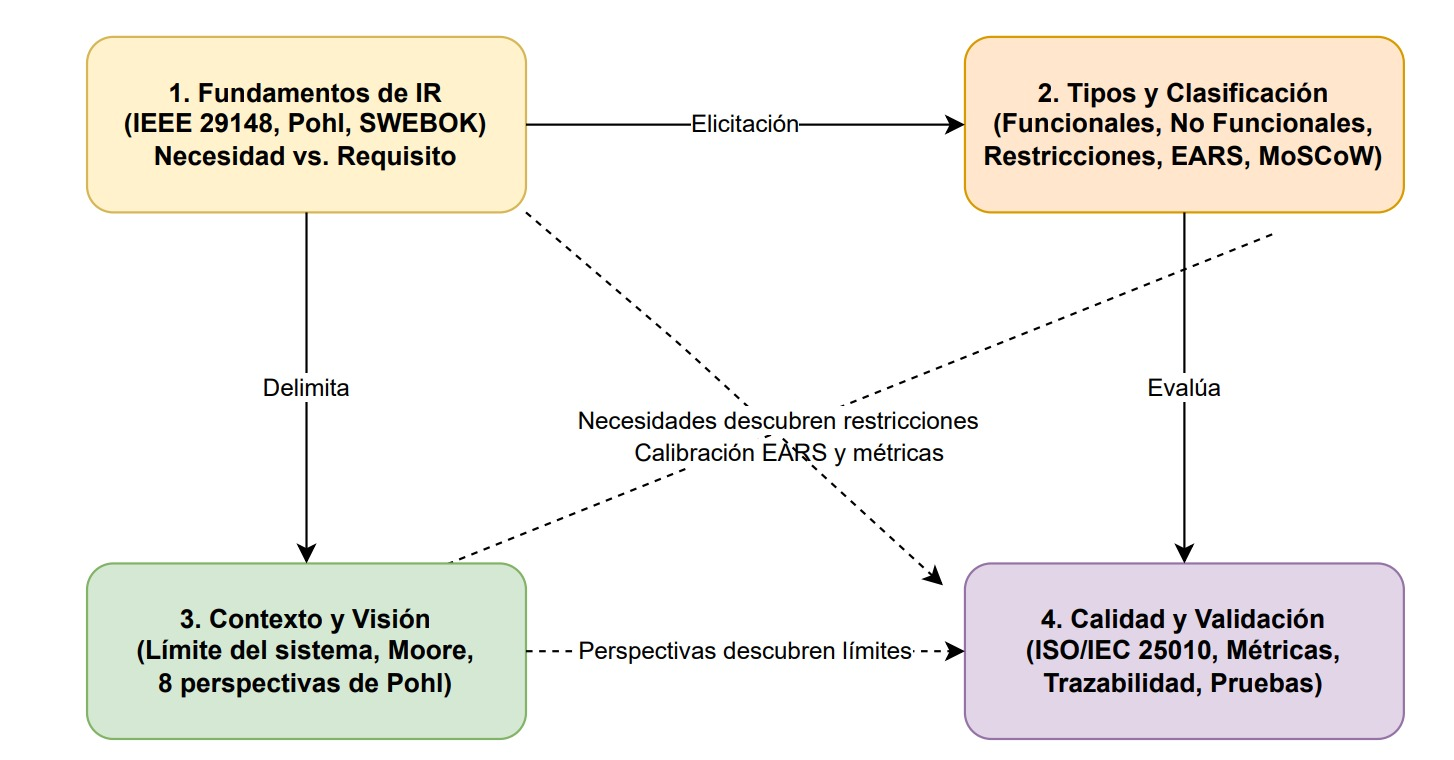
\includegraphics[
        width=10.80\linewidth,
        height=6.0cm,
        keepaspectratio
    ]{Figuras/DiagramaConceptual.jpeg}
}{
    \fbox{
        \parbox[c][3.5cm][c]{.72\linewidth}{
            \centering 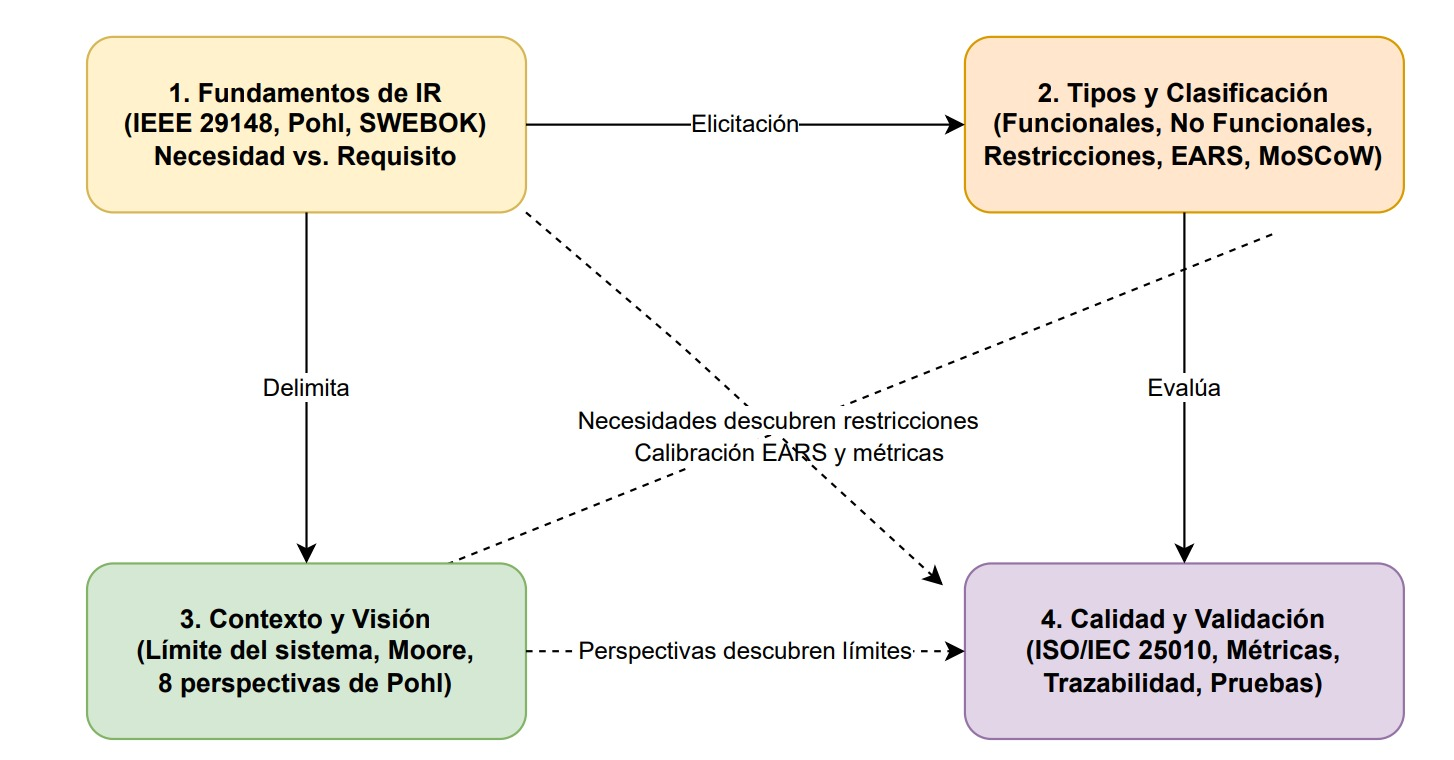
\includegraphics[width=4.95\linewidth, height=6.2cm, keepaspectratio]{Figuras/DiagramaConceptual.jpeg}        
        }
    }
}
\end{figure}
\textbf{Tres vínculos cruzados:} Necesidades $\rightarrow$ contexto; ISO 29148 $\rightarrow$ métricas; perspectivas de Pohl $\rightarrow$ restricciones. Estos enlaces se codifican como aristas discontinuas en la fuente editable de draw.io.


% ==================== 05_conclusiones ====================

\section{Conclusiones y control de entrega}
Las dos conclusiones se ofrecen como \textbf{textos de trabajo para revisión de cada integrante}, no como declaraciones ya aprobadas ni firmadas por ellos. Antes de publicar la versión final, cada estudiante debe revisarlas, ajustarlas con su criterio y poder defender la evidencia que emplea.

\subsection{Conclusión propuesta para Chalacán Toalá Yerai David}
\textbf{Afirmación.} El análisis de MEDICLAB evidencia que definir el alcance del sistema es indispensable para diferenciar una función informática de una responsabilidad clínica. \textbf{Evidencia.} Las capturas revelan módulos para pacientes, exámenes, órdenes, resultados y reportes; sin embargo, no prueban que la aplicación interprete diagnósticos ni que esté conectada con dispositivos de laboratorio. Esta distinción coincide con la importancia que Pohl atribuye al contexto y a los límites del sistema, así como con el carácter verificable de los requisitos de ISO/IEC/IEEE 29148:2018 \cite{pohl2025,iso29148}. \textbf{Implicación.} El equipo debe solicitar confirmación sobre los actores, las integraciones y el ciclo de vida de una orden antes de aprobar una especificación definitiva.

\subsection{Conclusión propuesta para Alvia Villegas Erick Adalberto}
\textbf{Afirmación.} La elaboración del catálogo demuestra que reconocer una opción de la interfaz no equivale a disponer de un requisito correctamente formulado. \textbf{Evidencia.} Los botones Agregar, Editar y Anular proporcionan indicios funcionales, mientras que una especificación necesita condiciones, respuestas y criterios de aceptación para comprobar cada obligación. La literatura de ingeniería de requisitos y la sintaxis EARS ayudan a separar el comportamiento esperado de las decisiones de implementación \cite{iso29148,mavin2009}. \textbf{Implicación.} Los identificadores, la priorización MoSCoW y la matriz de trazabilidad deberían mantenerse en el repositorio durante la evolución del proyecto, especialmente cuando una modificación de órdenes pueda afectar resultados, permisos o reportes.


\subsection{Verificación editorial y de integridad académica}
\begin{table}[H]\centering\small
\caption{Control objetivo previo a la publicación.}\label{tab:control}
\begin{tabularx}{\linewidth}{@{}Xp{3.0cm}@{}}\toprule
\textbf{Condición} & \textbf{Estado al generar este informe}\\\midrule
Sección 0 con equipo, descripción, tipo de sistema y 5 stakeholders simulados. & Elaborada; roles por aprobar.\\
Fundamento 2.1--2.6 con definiciones, interpretación y ejemplos. & Elaborado; títulos por contrastar con guía.\\
Matriz con mínimo 12 requisitos, fuentes, tipos y MoSCoW. & Elaborada: 20 candidatos.\\
Cinco requisitos de calidad con característica, métrica y umbral. & Elaborada: 5 propuestas.\\
Visión Moore, 5 entidades y límite funcional. & Elaborada; interfaces por verificar.\\
Ocho perspectivas con 3 preguntas y 2 candidatos cada una. & Elaborada: 24 preguntas + 16 candidatos.\\
Mapa conceptual editable con 3 vínculos cruzados. & Incluido en PDF y .drawio.\\
Capturas propias anonimizadas de MEDICLAB. & Incluidas en anexos.\\
Biblioteca Zotero/Mendeley y captura original del gestor. & PENDIENTE de evidencia real.\\
Revisión y conclusiones personales de cada estudiante. & PENDIENTE de aprobación del equipo.\\
Repositorio público, URL y hoja SGA definitiva. & PENDIENTE de publicación.\\\bottomrule
\end{tabularx}
\end{table}

\subsection{Declaración de apoyo mediante inteligencia artificial}
\textbf{Herramienta:} ChatGPT de OpenAI, Gemini. \textbf{Propósito:} apoyo en análisis de capturas del prototipo, consulta de bibliografía, organización de categorías,Guia para elaboración de fuente LaTeX. \textbf{Verificación realizada:} cotejo inicial con las capturas del proyecto suministradas, confirmación de datos editoriales de referencias brindadas por el usuario. \textbf{Pendiente de verificación humana:} exactitud de la implementación y revisión de las normas completas. No se han inventado entrevistas, pruebas de rendimiento ni acuerdos de interesados.

\clearpage
\bibliographystyle{IEEEtran}
\bibliography{referencias}
\clearpage
\appendix

% ==================== 06_anexos ====================
\section{Anexo A. Evidencias de interfaz}
Las siguientes figuras proceden de las capturas del programa proporcionadas por un miembro del equipo. cabe recalcar que para esta muestra academica se usaron nombres de pacientes ficticios que no representan ningun problema medico. Su presencia es puramente para prueba de elementos visuales y academicas, no de ejecución satisfactoria de operaciones.

\begin{figure}[H]\centering
\IfFileExists{}{
    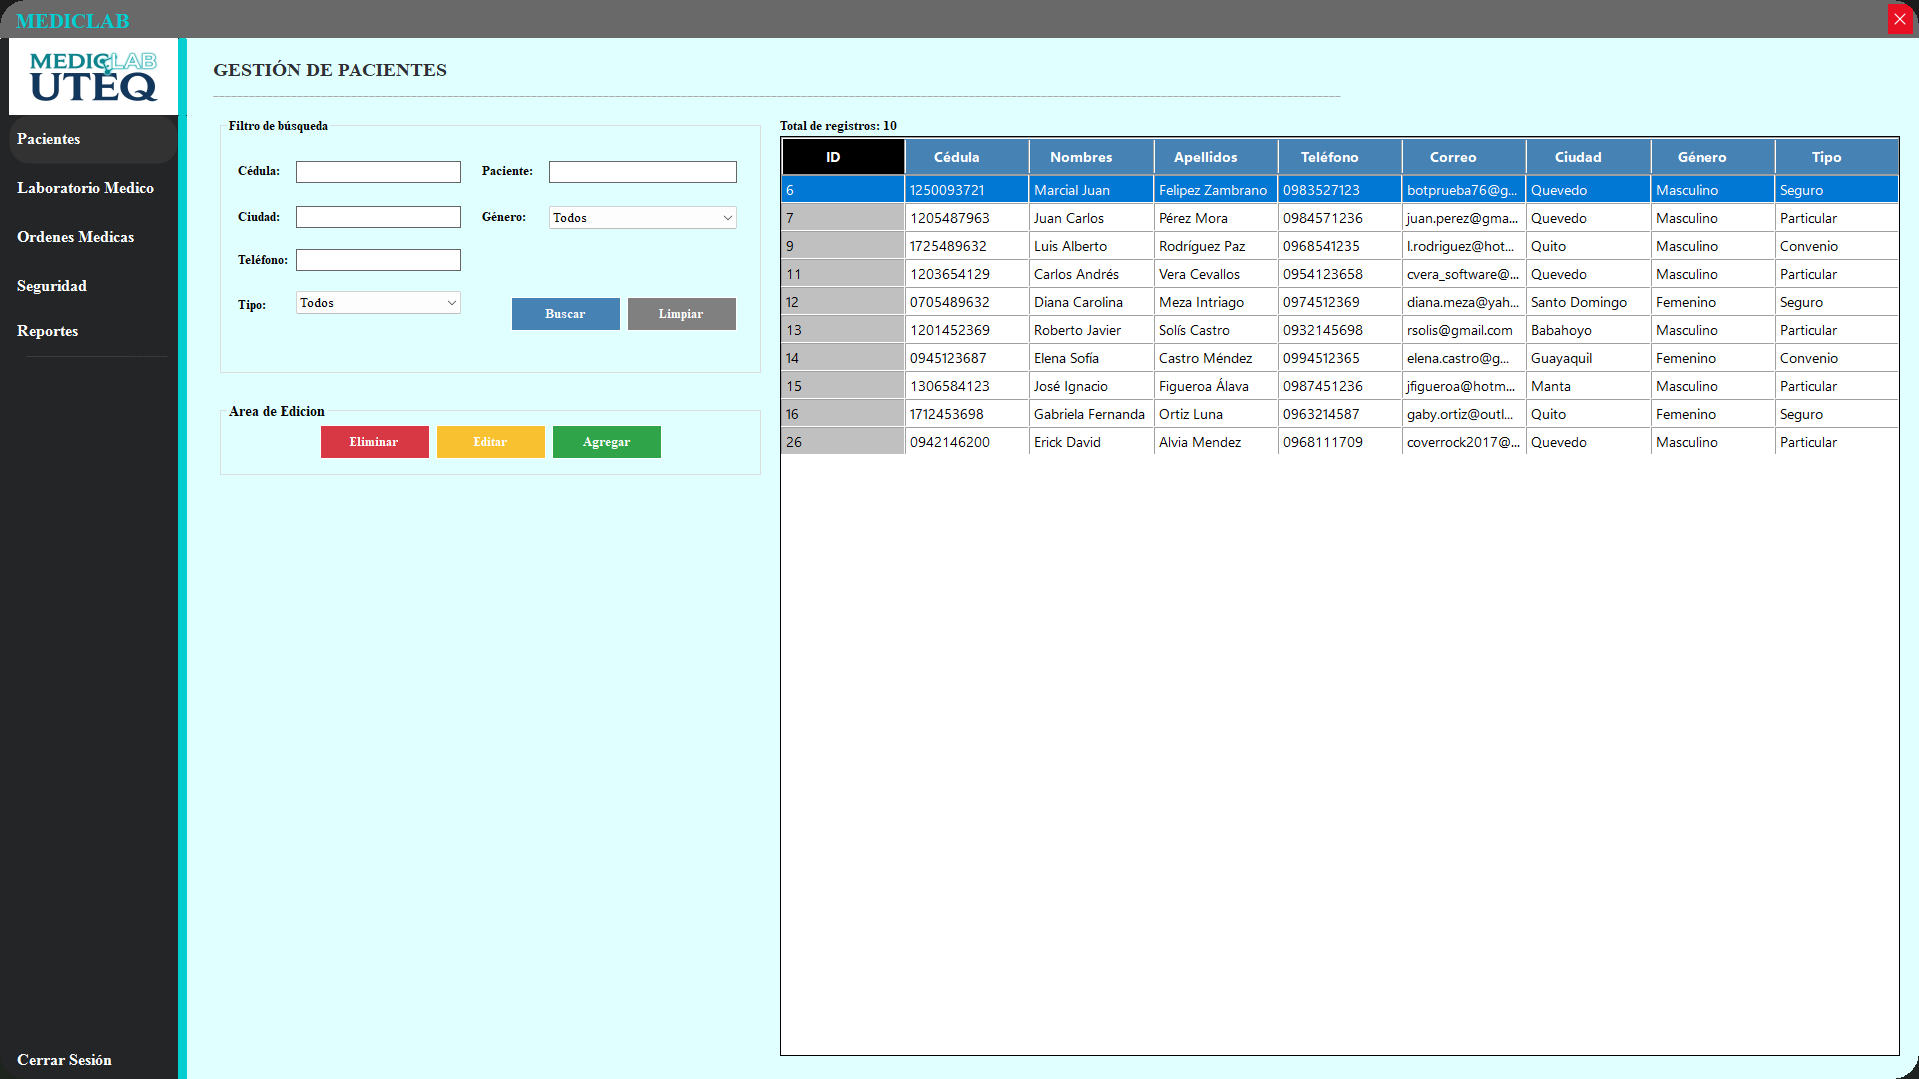
\includegraphics[
        width=9.80\linewidth,
        height=7.0cm,
        keepaspectratio
    ]{Evidencia_Interfaz/Pacientes_01.png}
}{
    \fbox{
        \parbox[c][6.5cm][c]{.72\linewidth}{
            \centering 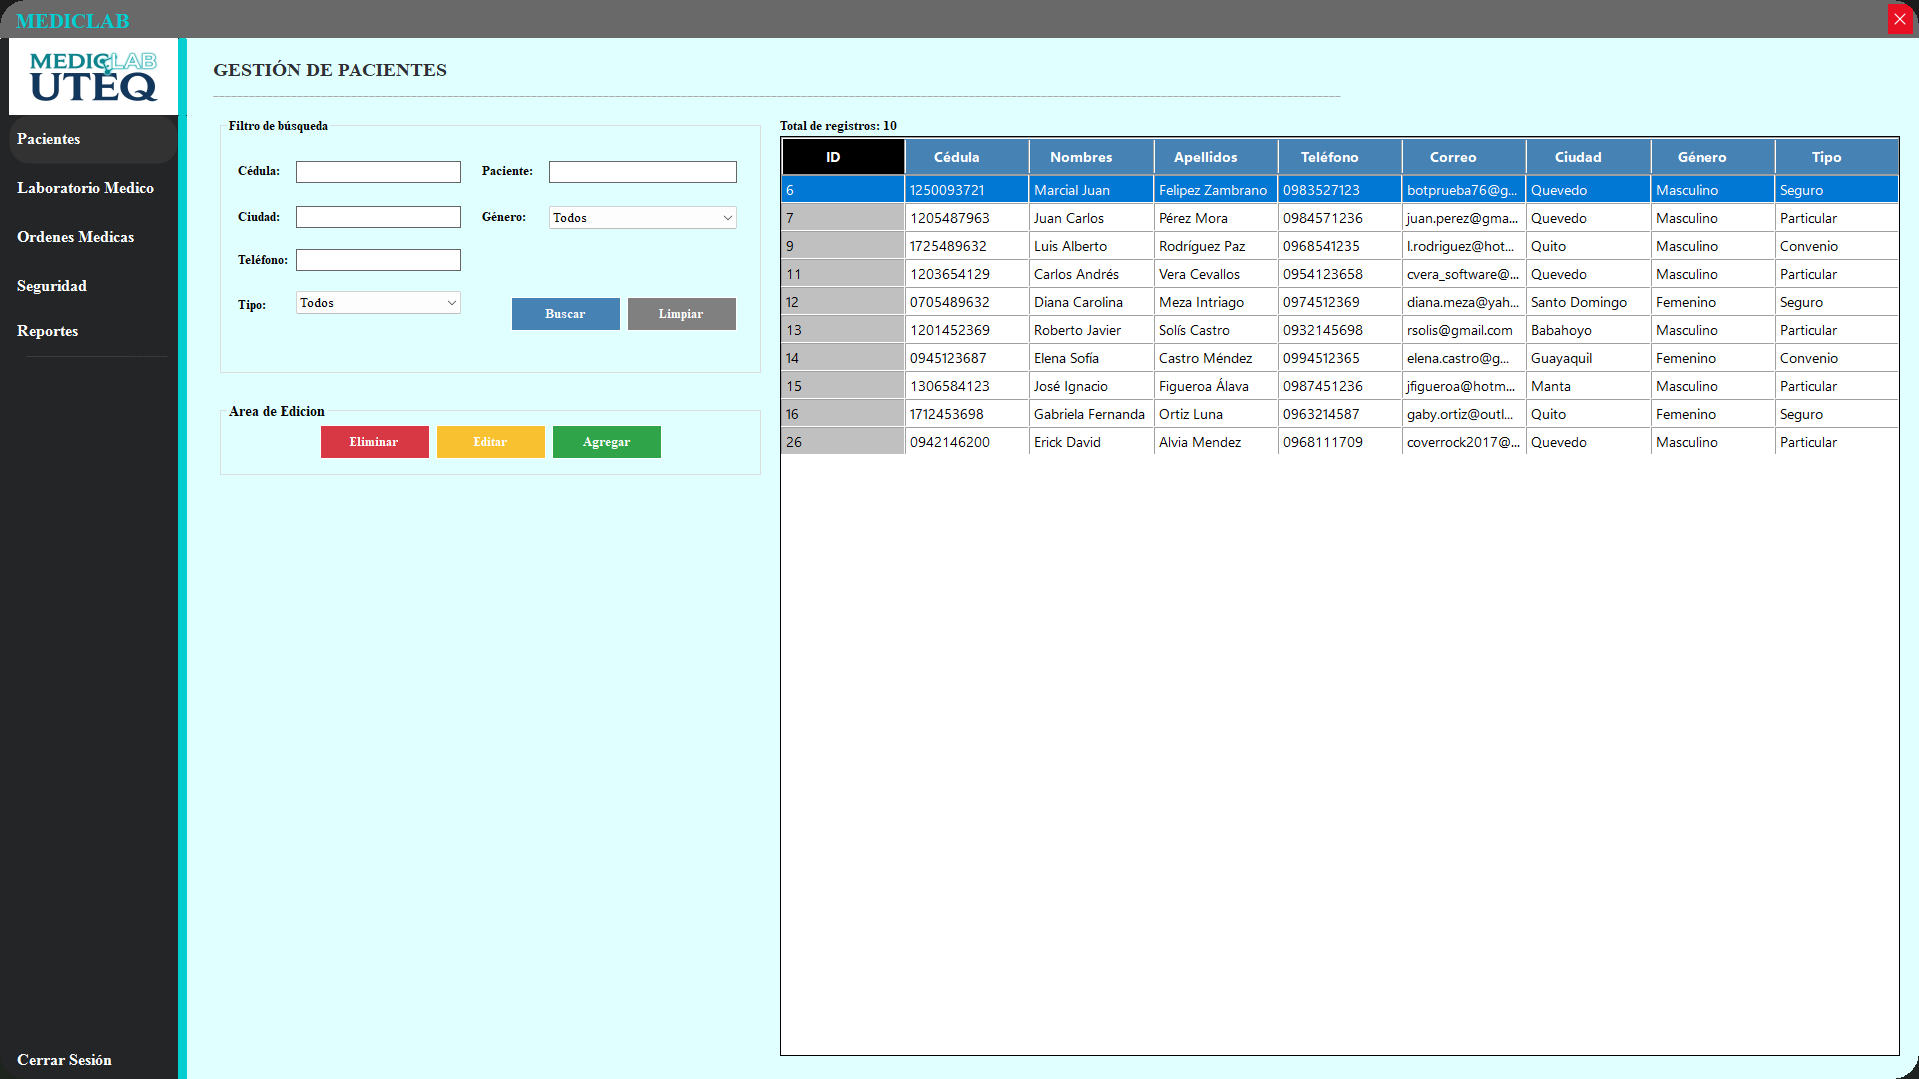
\includegraphics[width=4.95\linewidth, height=6.2cm, keepaspectratio]{Evidencia_Interfaz/Pacientes_01.png}        
        }
    }
}

\caption{Gestión de pacientes y filtros; filas con datos personales ocultas. Apoyo a RF-01, RF-02 y US-01.}\label{fig:Pacientes_01}\end{figure}

\begin{figure}[H]\centering
\IfFileExists{}{
    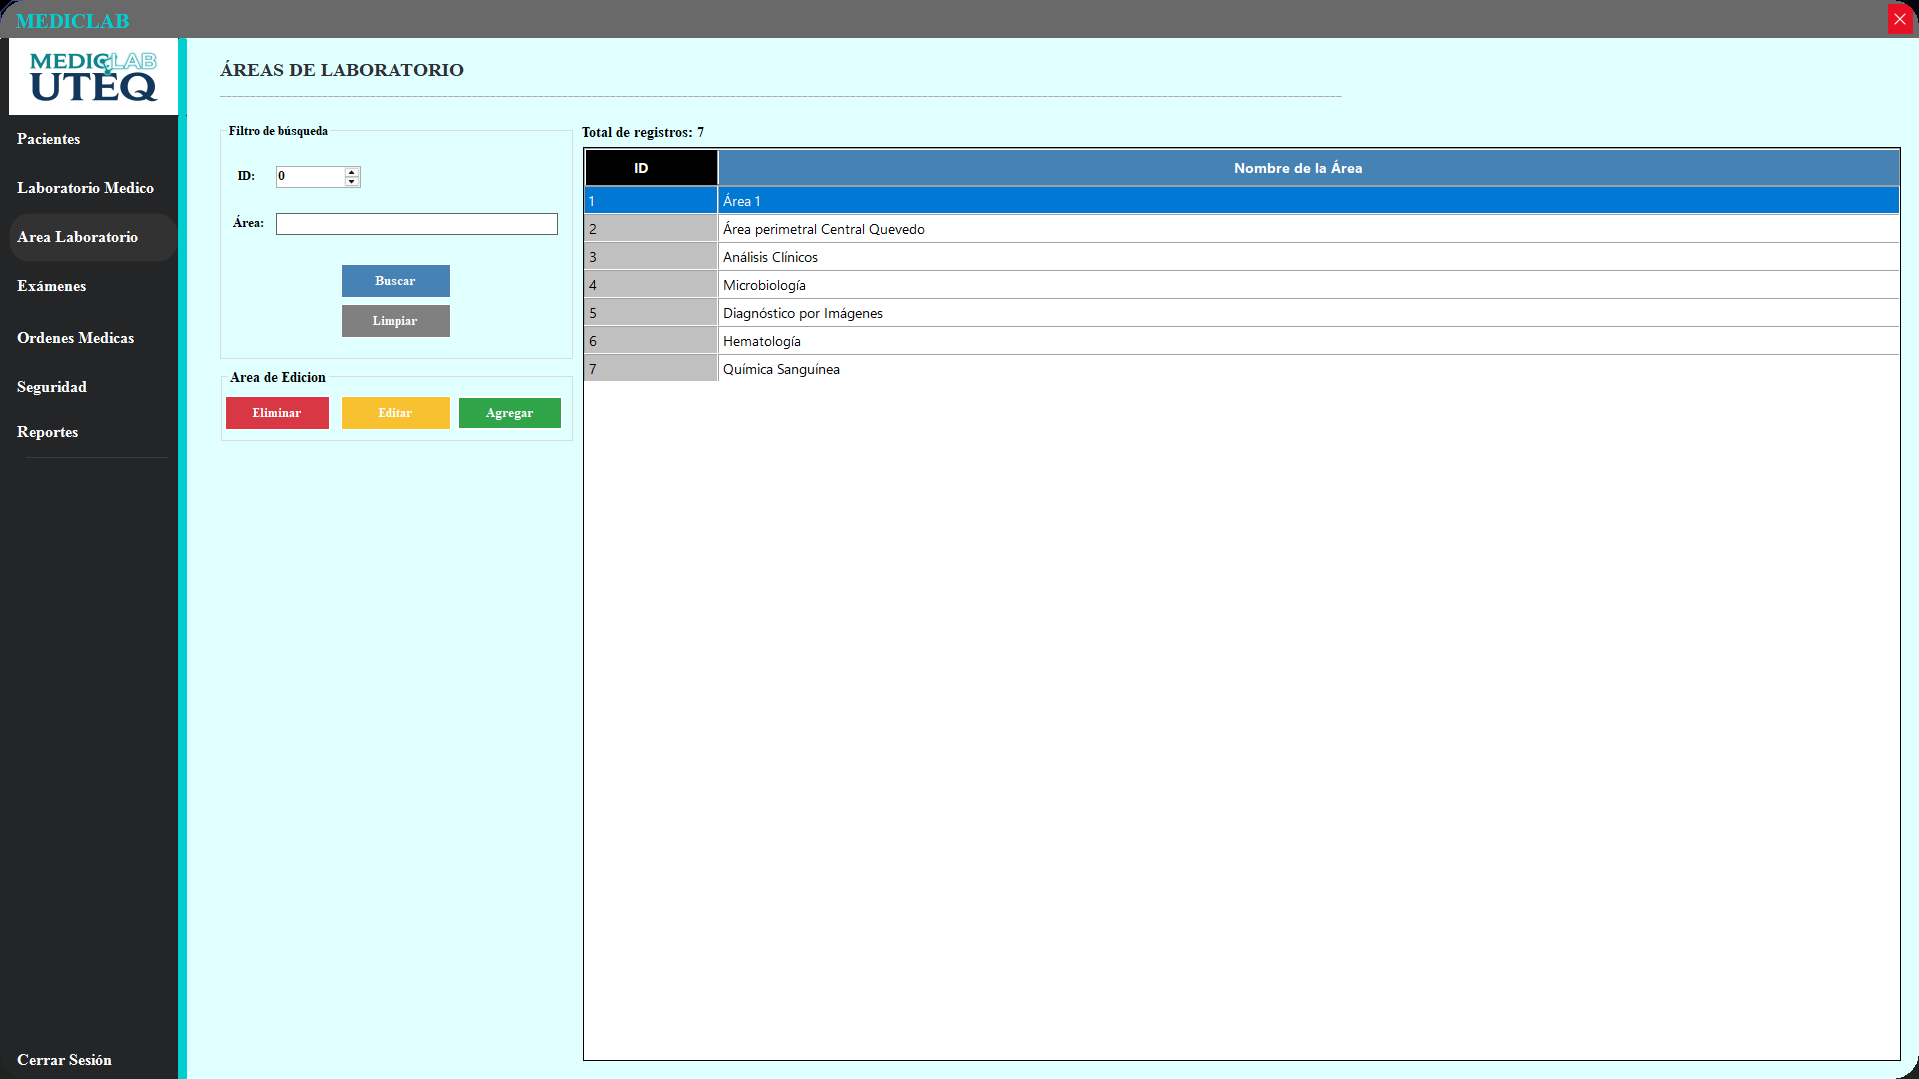
\includegraphics[
        width=9.80\linewidth,
        height=7.0cm,
        keepaspectratio
    ]{Evidencia_Interfaz/areas_02.png}
}{
    \fbox{
        \parbox[c][6.5cm][c]{.72\linewidth}{
            \centering 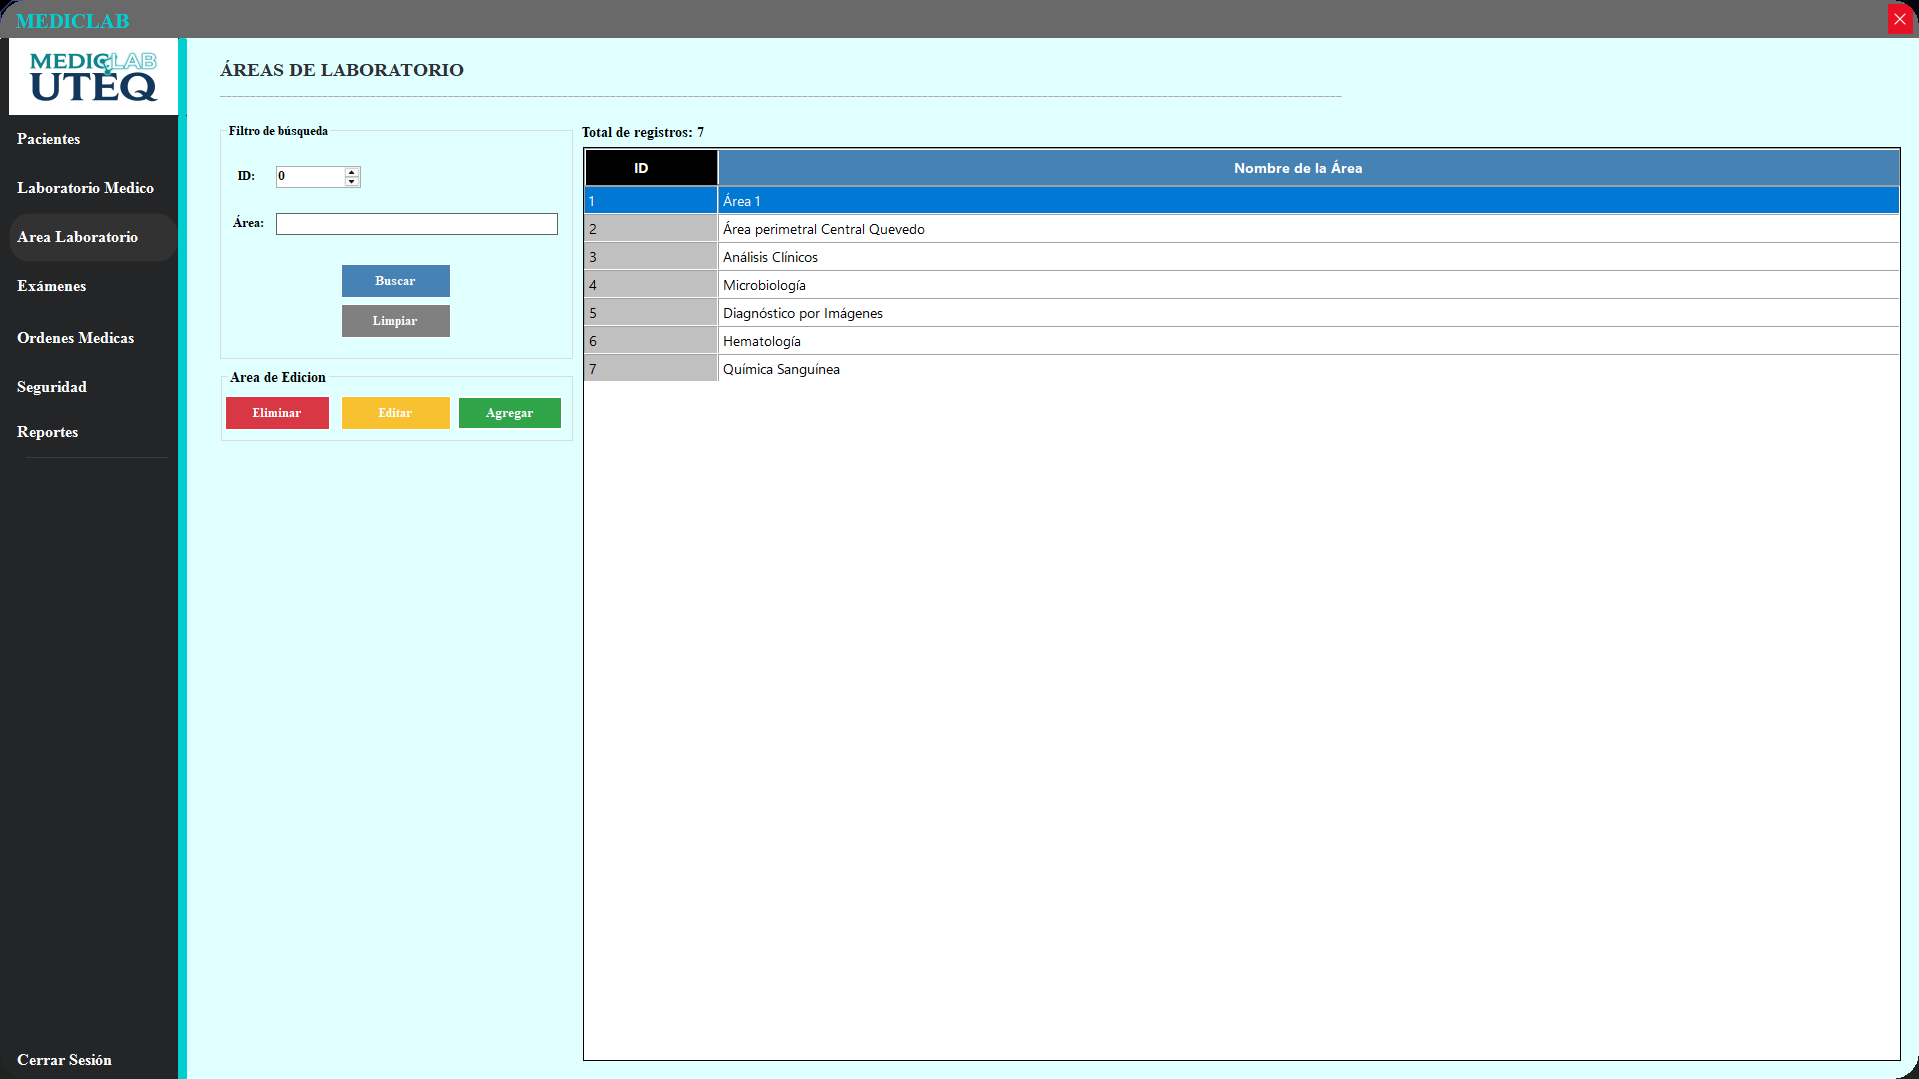
\includegraphics[width=4.95\linewidth, height=6.2cm, keepaspectratio]{Evidencia_Interfaz/areas_02.png}        
        }
    }
}\caption{Catálogo de áreas de laboratorio y acciones de edición. Apoyo a RF-03.}\label{fig:areas_02}\end{figure}

\begin{figure}[H]\centering
\IfFileExists{}{
    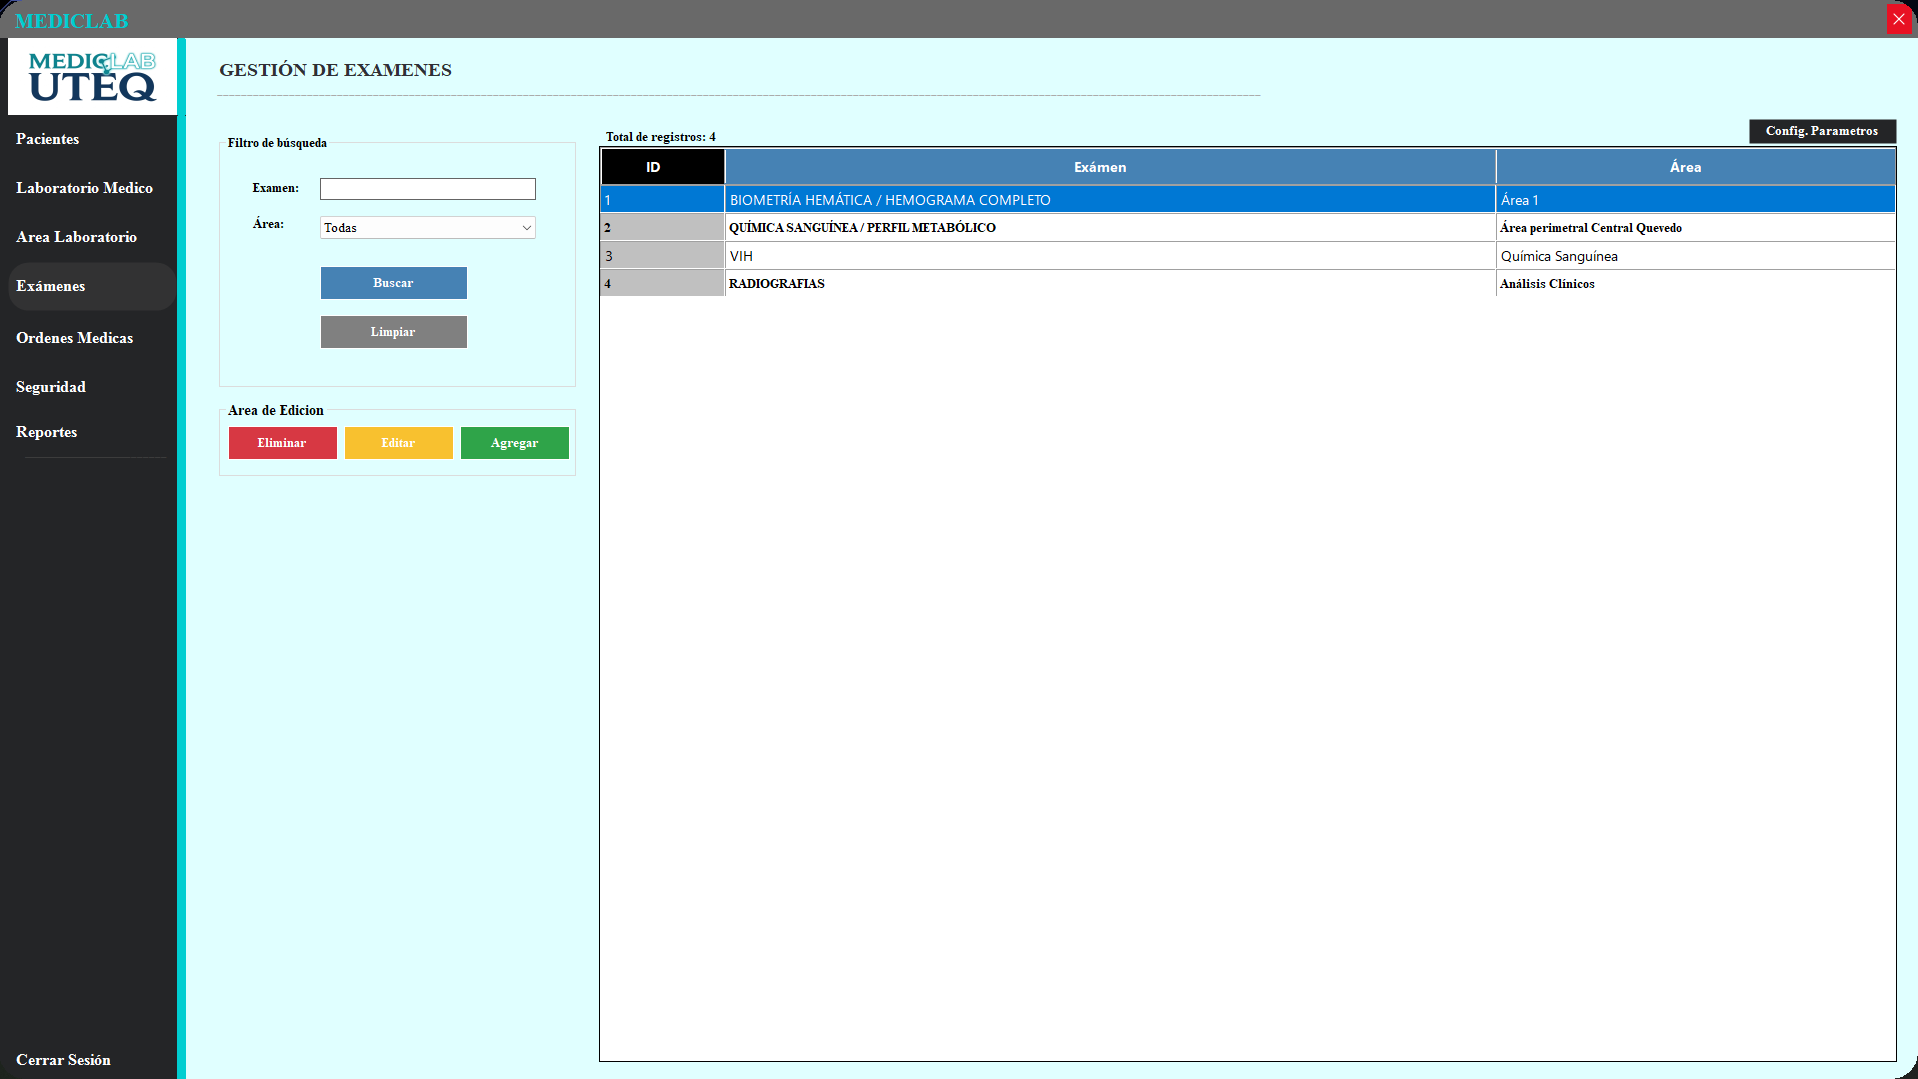
\includegraphics[
        width=9.80\linewidth,
        height=7.0cm,
        keepaspectratio
    ]{Evidencia_Interfaz/Examenes_03.png}
}{
    \fbox{
        \parbox[c][6.5cm][c]{.72\linewidth}{
            \centering 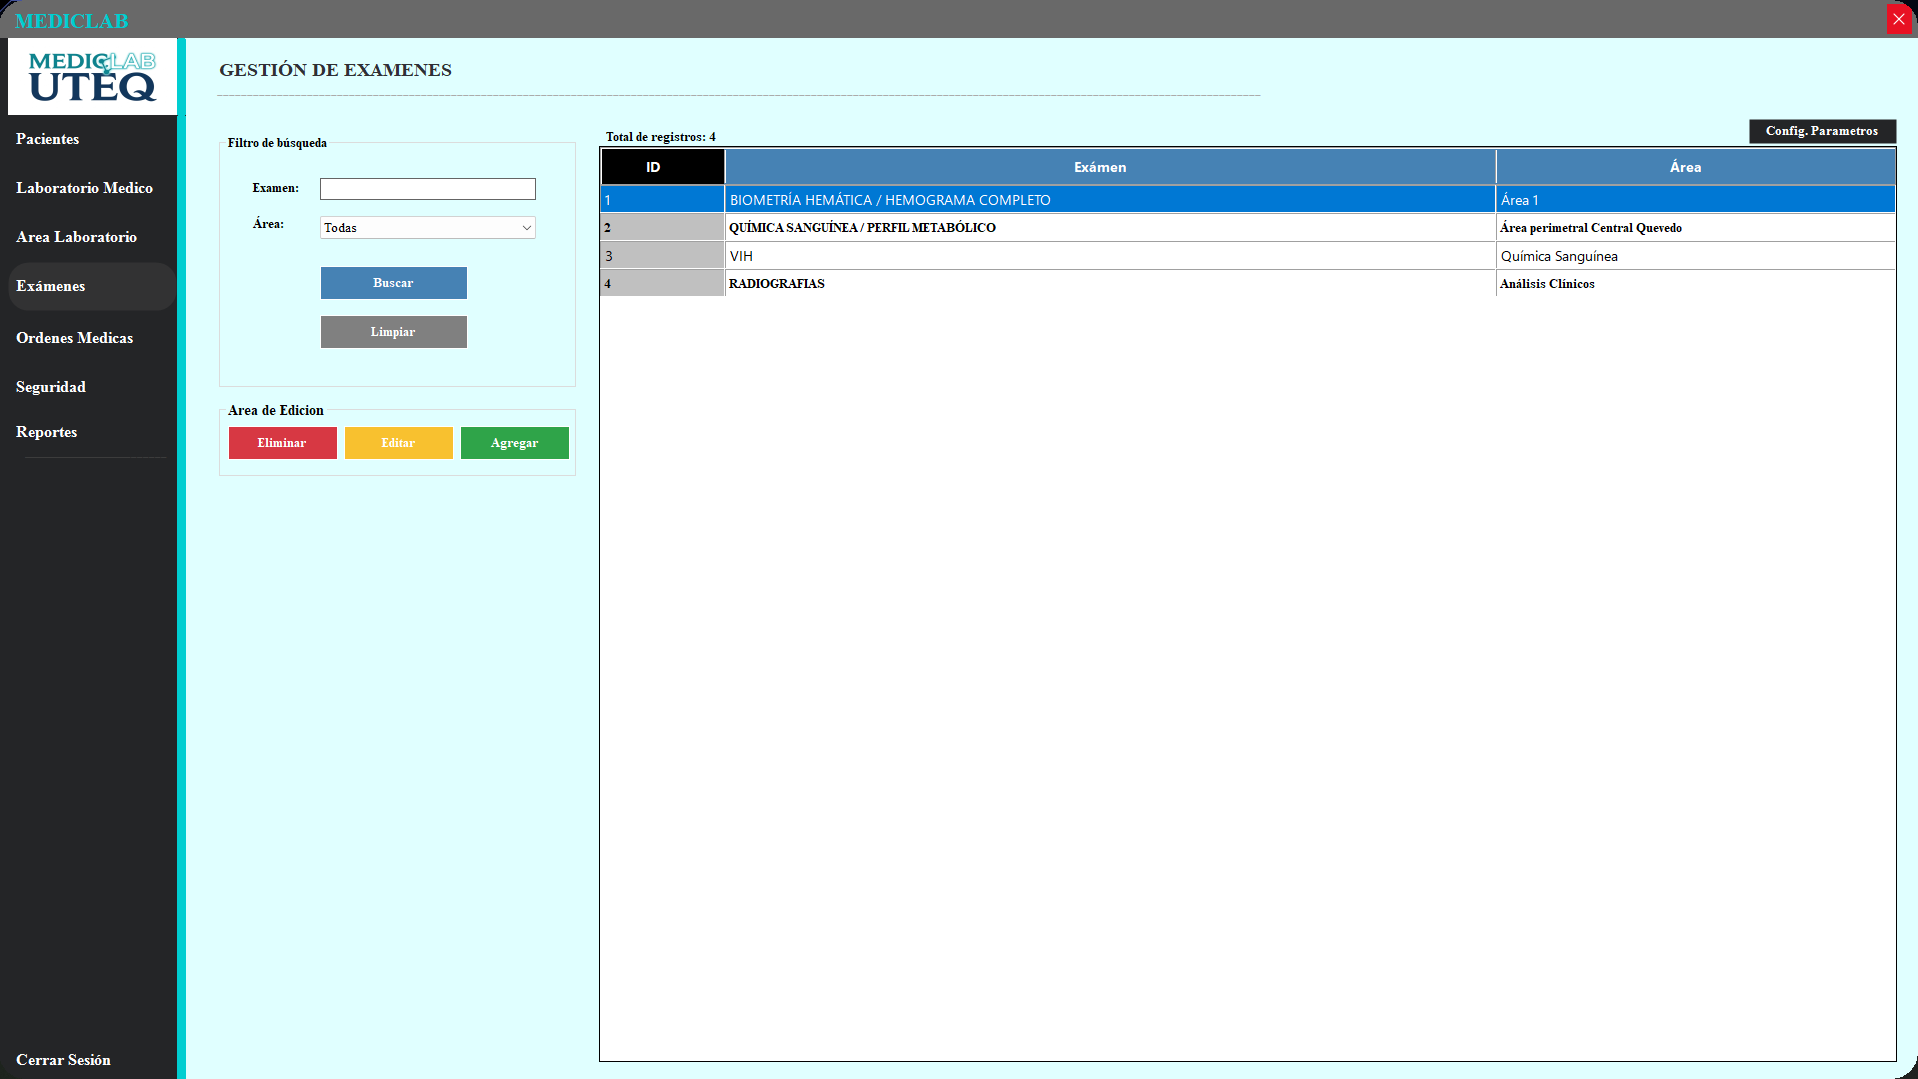
\includegraphics[width=4.95\linewidth, height=6.2cm, keepaspectratio]{Evidencia_Interfaz/Examenes_03.png}        
        }
    }
}\caption{Catálogo de exámenes asociado a áreas. Apoyo a RF-04.}\label{fig:Examenes_03}\end{figure}

\begin{figure}[H]\centering
\IfFileExists{}{
    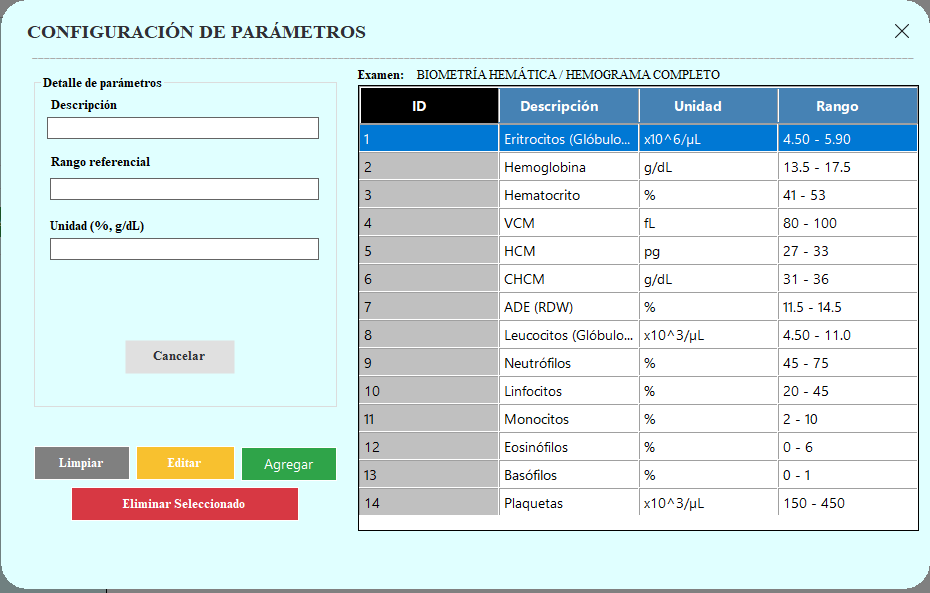
\includegraphics[
        width=9.80\linewidth,
        height=7.0cm,
        keepaspectratio
    ]{Evidencia_Interfaz/Parametros_04.png}
}{
    \fbox{
        \parbox[c][6.5cm][c]{.72\linewidth}{
            \centering 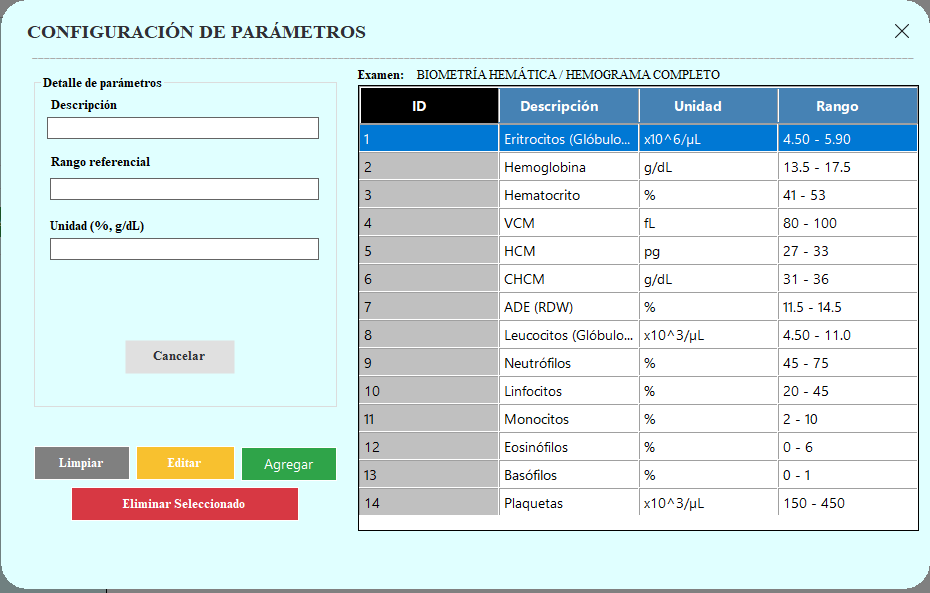
\includegraphics[width=4.95\linewidth, height=6.2cm, keepaspectratio]{Evidencia_Interfaz/Parametros_04.png}        
        }
    }
}\caption{Formulario y catálogo de parámetros de examen: descripción, unidad y rango. Apoyo a RF-05.}\label{fig:Parametros_04}\end{figure}

\begin{figure}[H]\centering
\IfFileExists{}{
    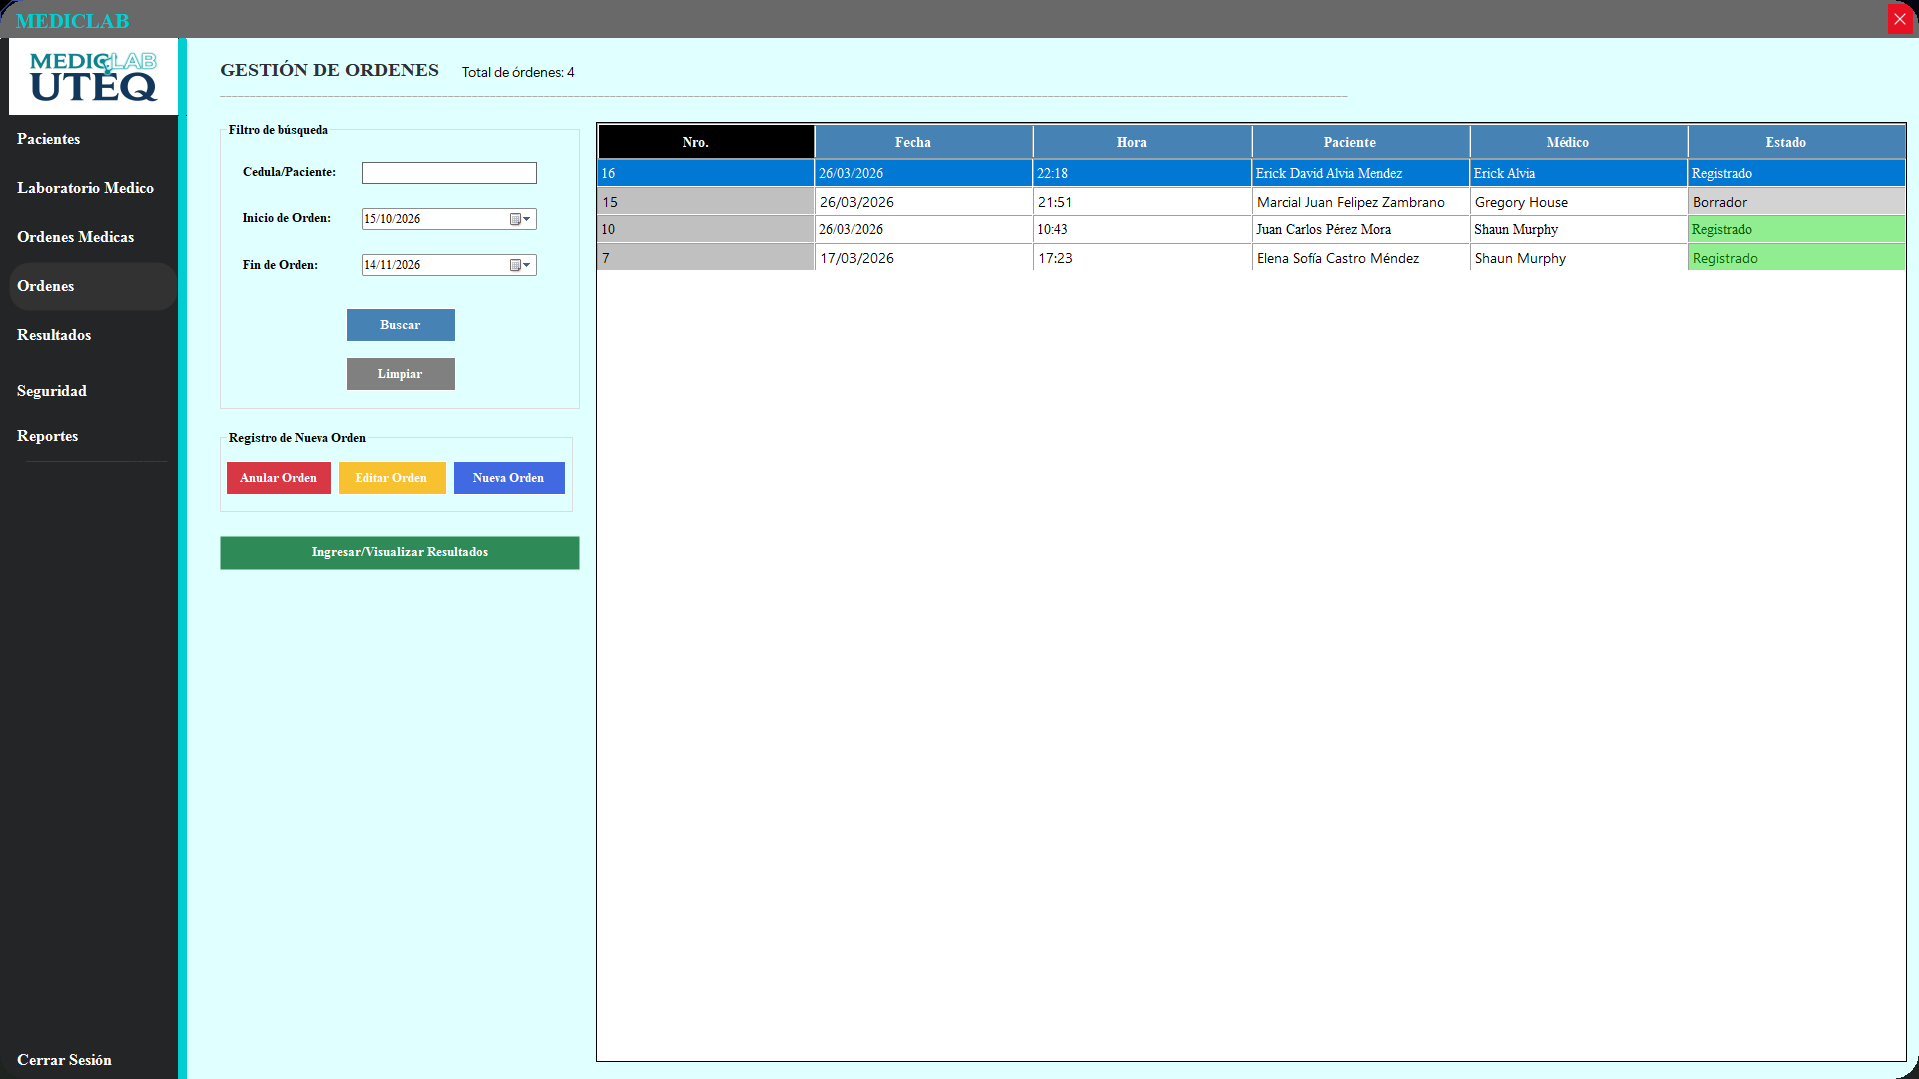
\includegraphics[
        width=9.80\linewidth,
        height=7.0cm,
        keepaspectratio
    ]{Evidencia_Interfaz/Ordenes_05.png}
}{
    \fbox{
        \parbox[c][6.5cm][c]{.72\linewidth}{
            \centering 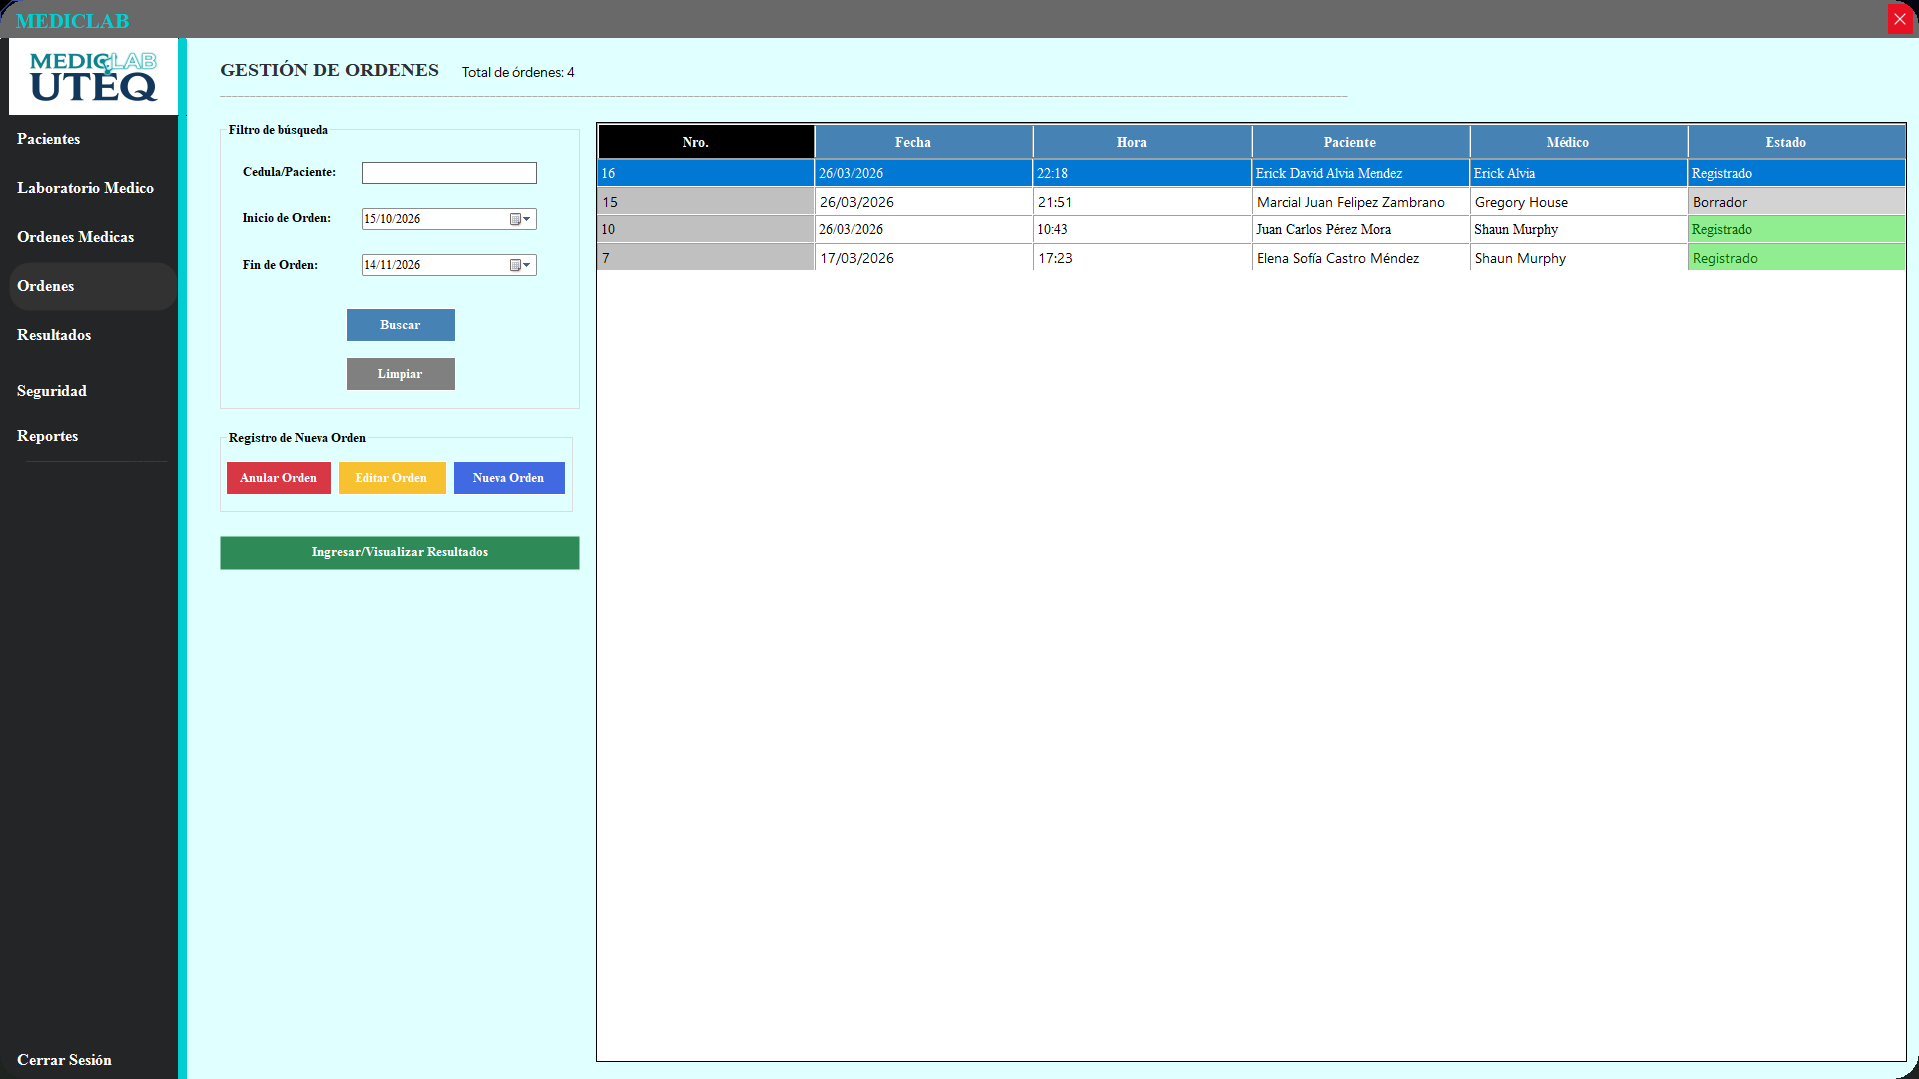
\includegraphics[width=4.95\linewidth, height=6.2cm, keepaspectratio]{Evidencia_Interfaz/Ordenes_05.png}        
        }
    }
}\caption{Gestión de órdenes y acciones visibles; información personal oculta. Apoyo a RF-06 y RF-07.}\label{fig:Ordenes_05}\end{figure}

\begin{figure}[H]\centering
\IfFileExists{}{
    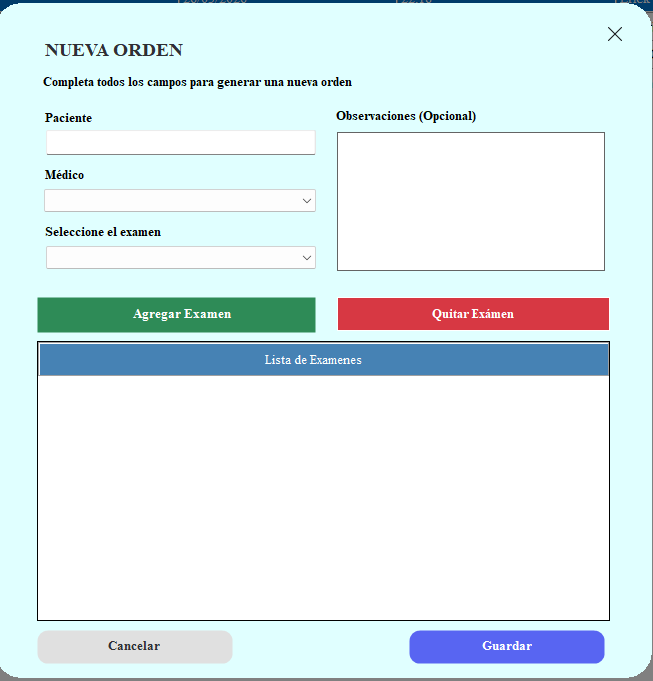
\includegraphics[
        width=9.80\linewidth,
        height=7.0cm,
        keepaspectratio
    ]{Evidencia_Interfaz/Nueva_orden_06.png}
}{
    \fbox{
        \parbox[c][6.5cm][c]{.72\linewidth}{
            \centering 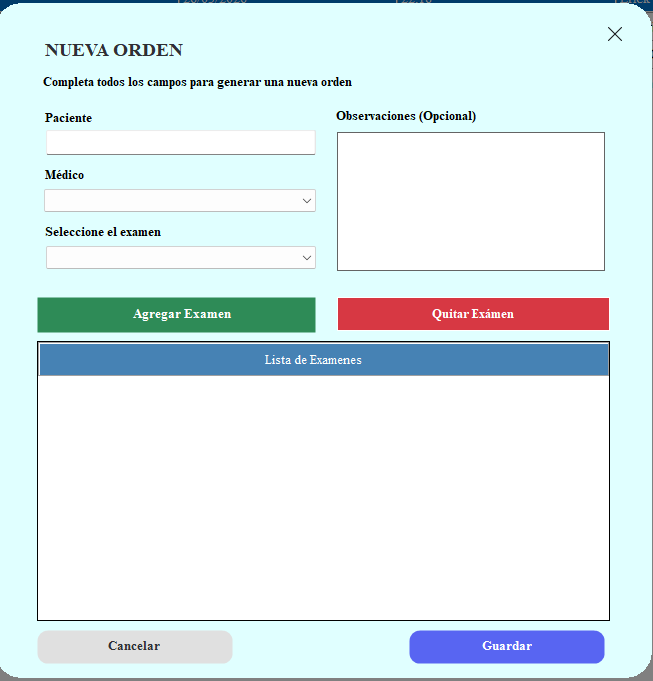
\includegraphics[width=4.95\linewidth, height=6.2cm, keepaspectratio]{Evidencia_Interfaz/Nueva_orden_06.png}        
        }
    }
}\caption{Formulario de nueva orden con selección de paciente, médico y examen. Apoyo a RF-06.}\label{fig:Nueva_orden_06}\end{figure}

\begin{figure}[H]\centering
\IfFileExists{}{
    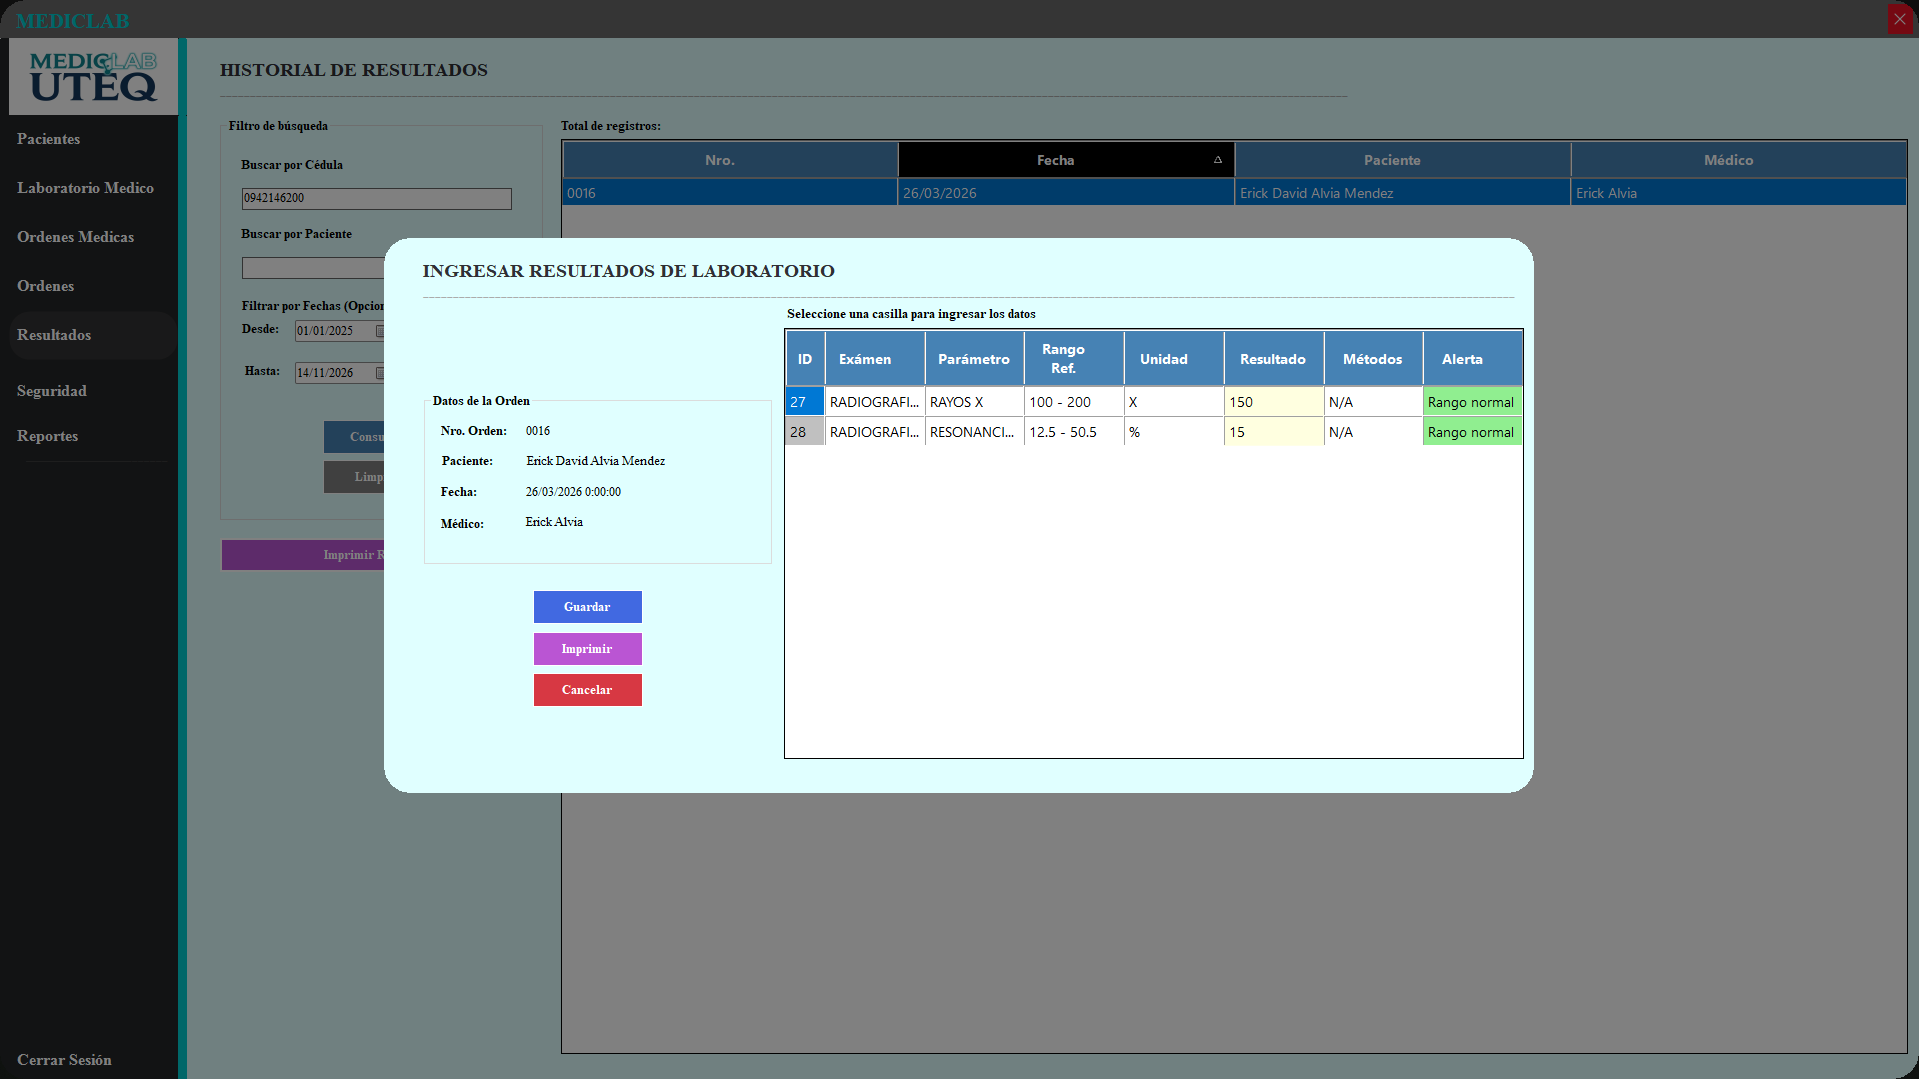
\includegraphics[
        width=9.80\linewidth,
        height=7.0cm,
        keepaspectratio
    ]{Evidencia_Interfaz/Resultados_07.png}
}{
    \fbox{
        \parbox[c][6.5cm][c]{.72\linewidth}{
            \centering 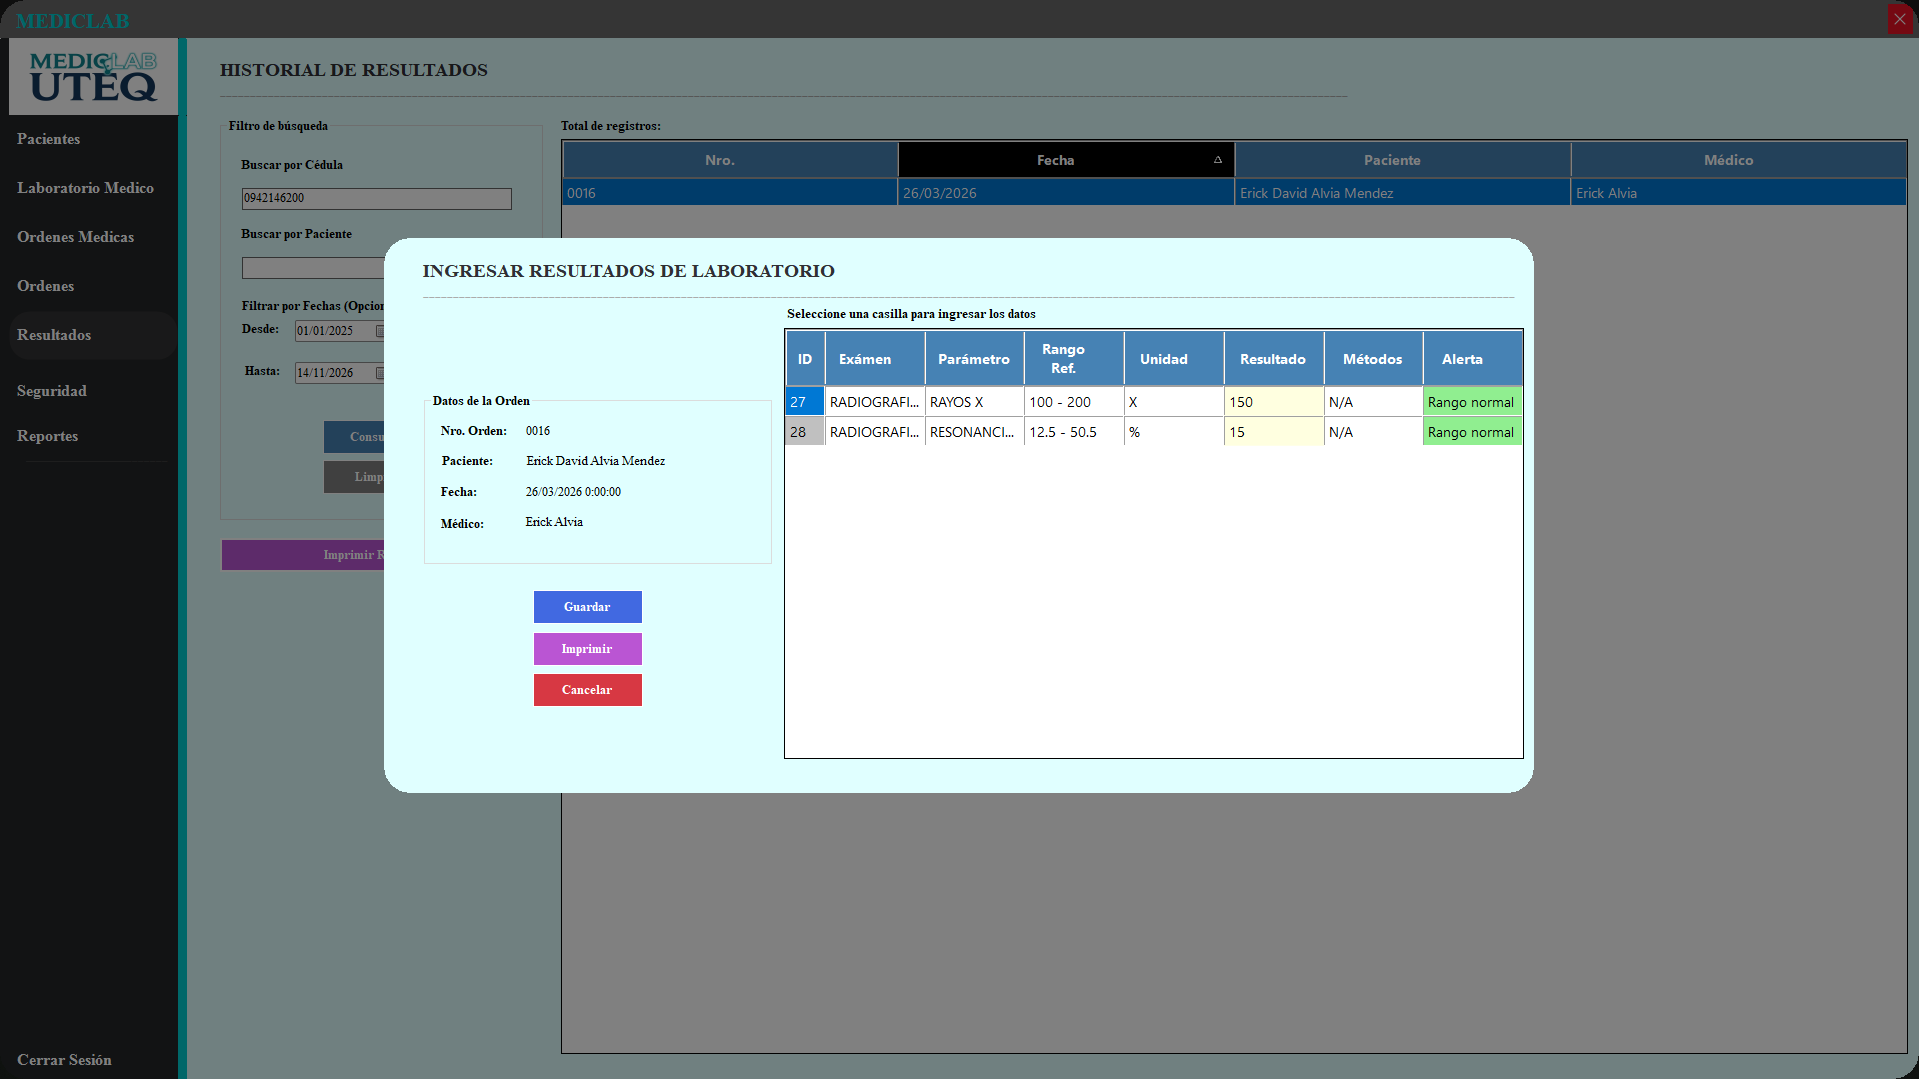
\includegraphics[width=4.95\linewidth, height=6.2cm, keepaspectratio]{Evidencia_Interfaz/Resultados_07.png}        
        }
    }
}\caption{Historial de resultados y filtros. Apoyo a RF-08; no demuestra disponibilidad de resultados en la muestra.}\label{fig:Resultados_07}\end{figure}

\begin{figure}[H]\centering
\IfFileExists{}{
    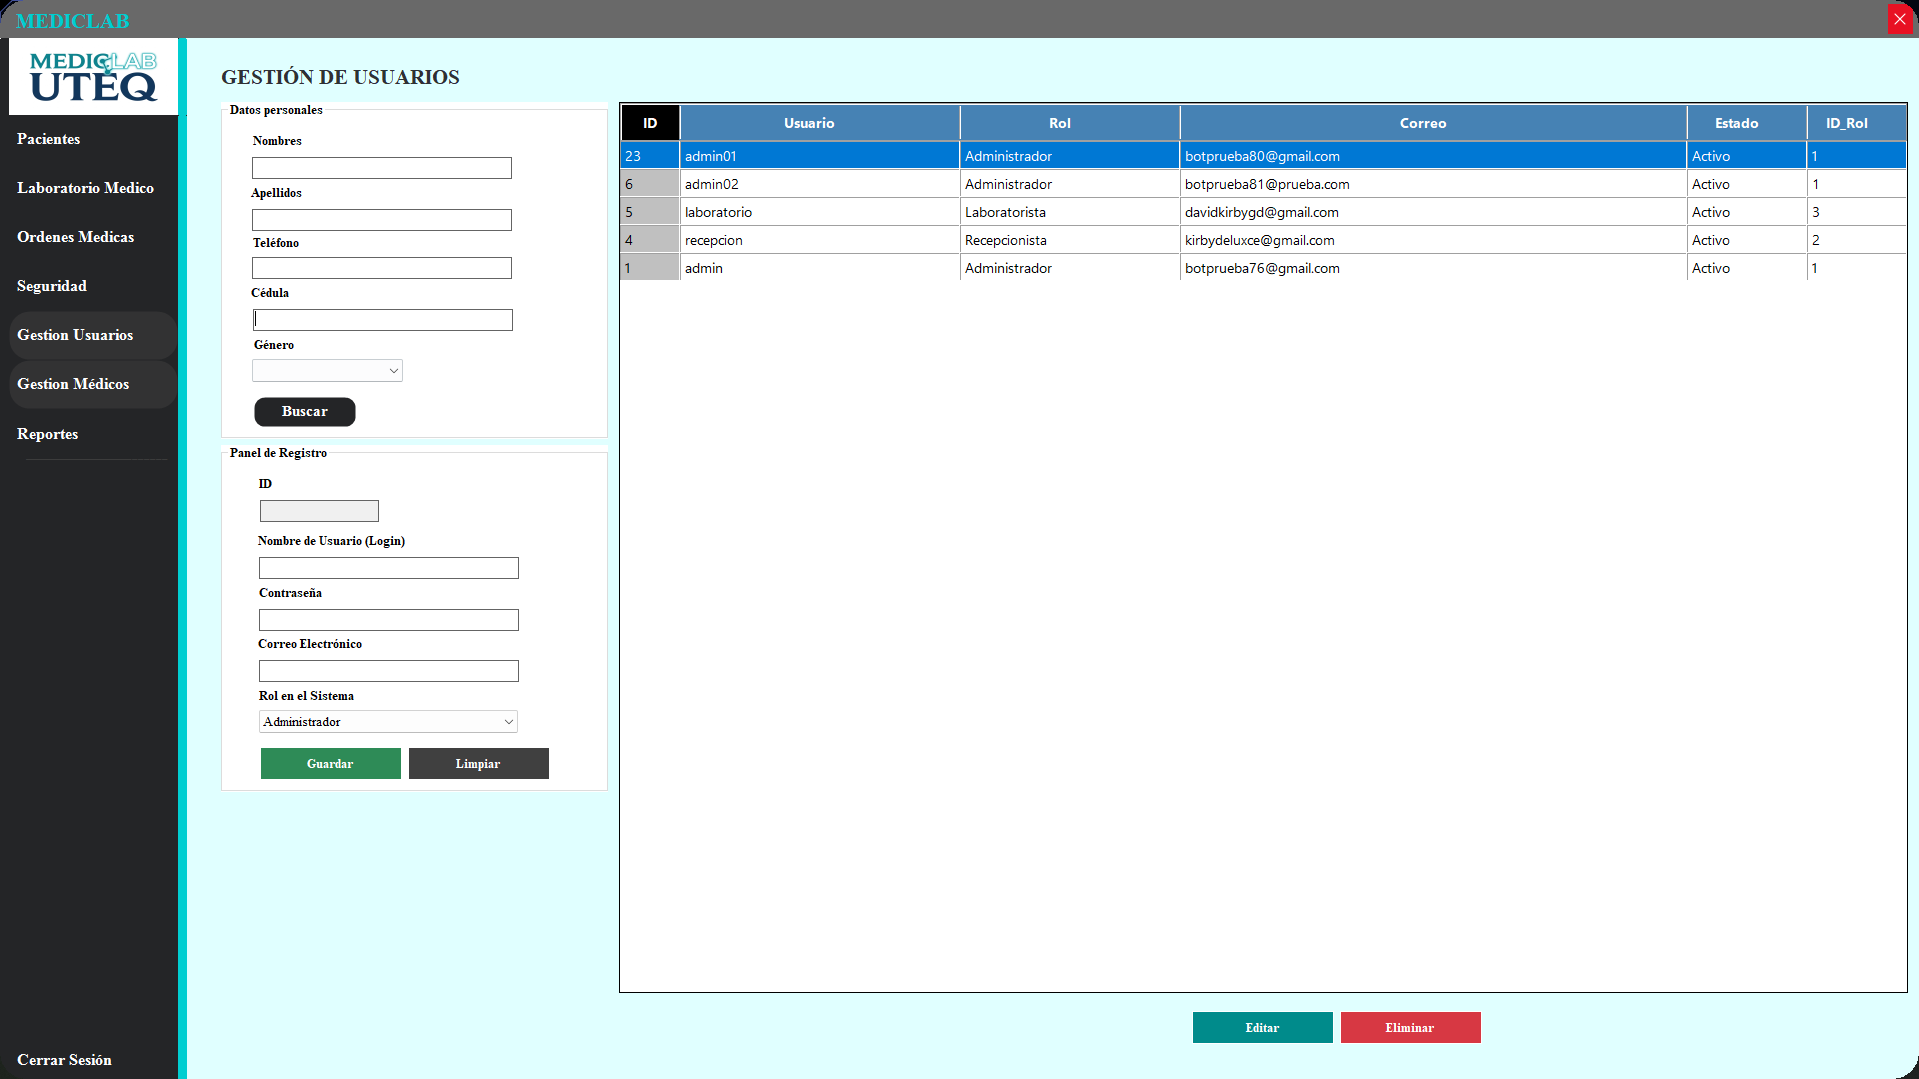
\includegraphics[
        width=9.80\linewidth,
        height=7.0cm,
        keepaspectratio
    ]{Evidencia_Interfaz/Usuarios_08.png}
}{
    \fbox{
        \parbox[c][6.5cm][c]{.72\linewidth}{
            \centering 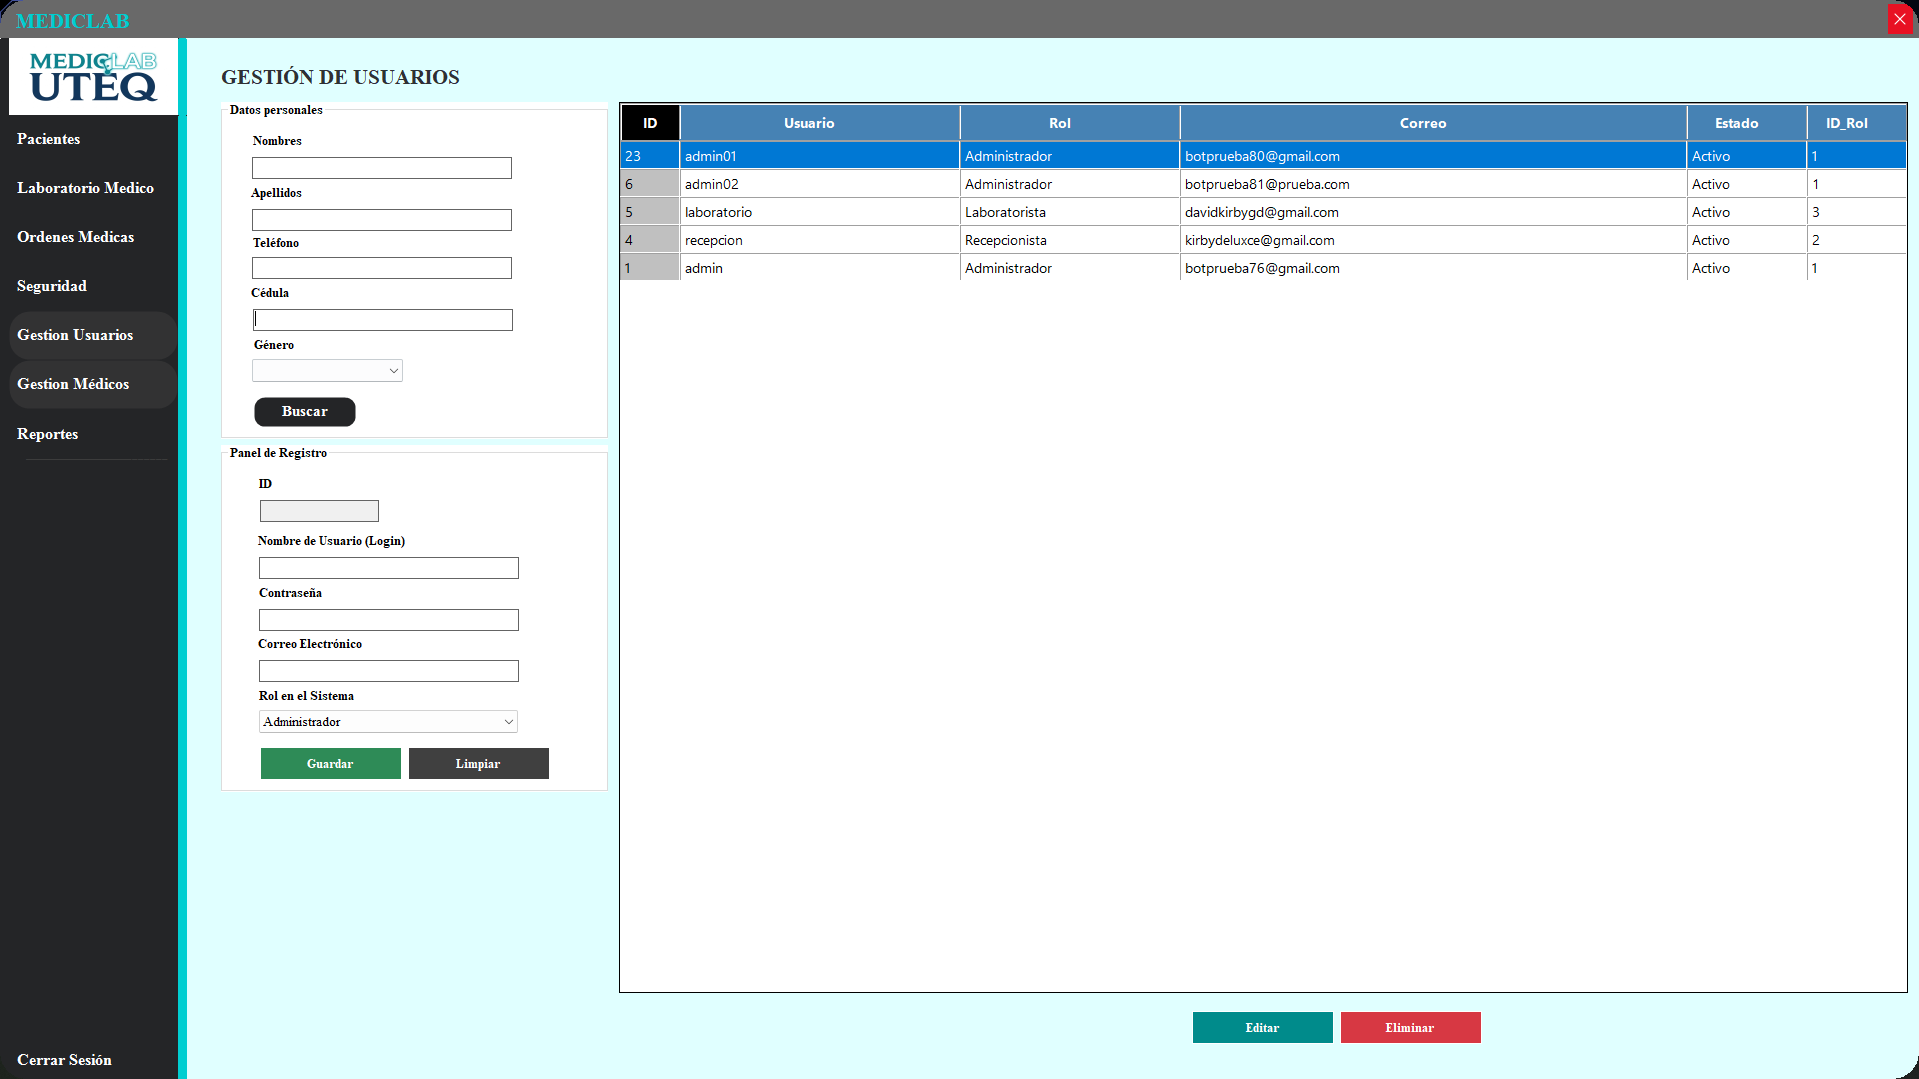
\includegraphics[width=4.95\linewidth, height=6.2cm, keepaspectratio]{Evidencia_Interfaz/Usuarios_08.png}        
        }
    }
}\caption{Gestión de cuentas, roles y formulario de registro; filas identificativas ocultas. Apoyo al análisis de seguridad.}\label{fig:Usuarios_08}\end{figure}


\section{Anexo B. Registro de evidencias y fuentes reproducibles}

\textbf{Evidencia Aportada de captura de fuentes en Mendeley:} captura de Zotero/Mendeley con el registro real de las fuentes. Debe obtenerse desde la biblioteca del equipo, nunca generarse o simularse. Igualmente, cualquier captura nueva con datos de pacientes deberá anonimizarse antes de su publicación.

\begin{figure}[H]\centering
\IfFileExists{}{
    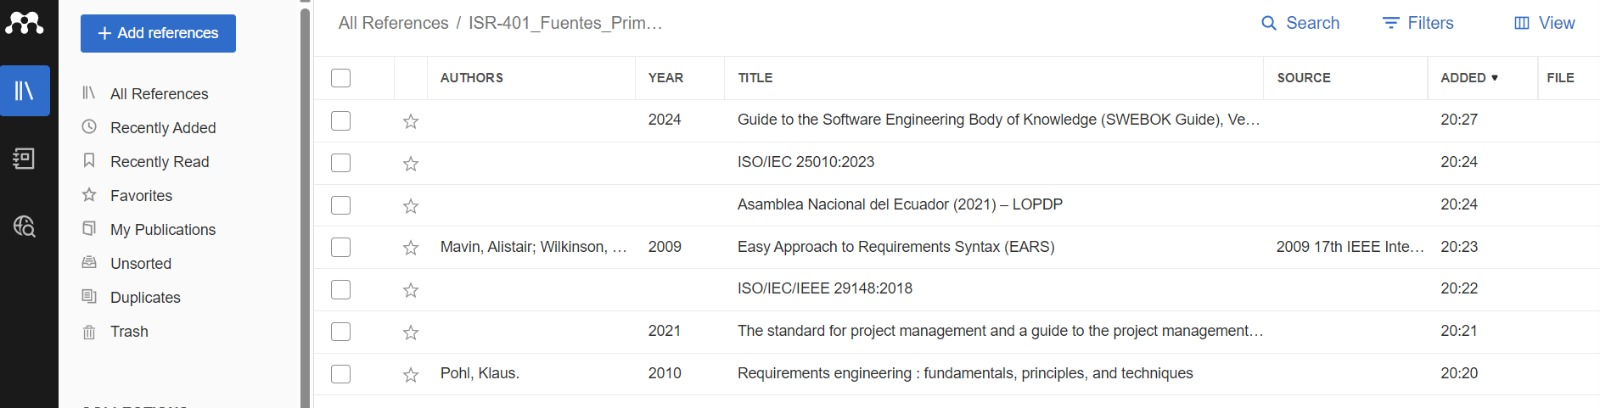
\includegraphics[
        width=6.80\linewidth,
        height=4.5cm,
        keepaspectratio
    ]{Figuras/Evidencia_mendeley.jpeg}
}{
    \fbox{
        \parbox[c][6.5cm][c]{.72\linewidth}{
            \centering 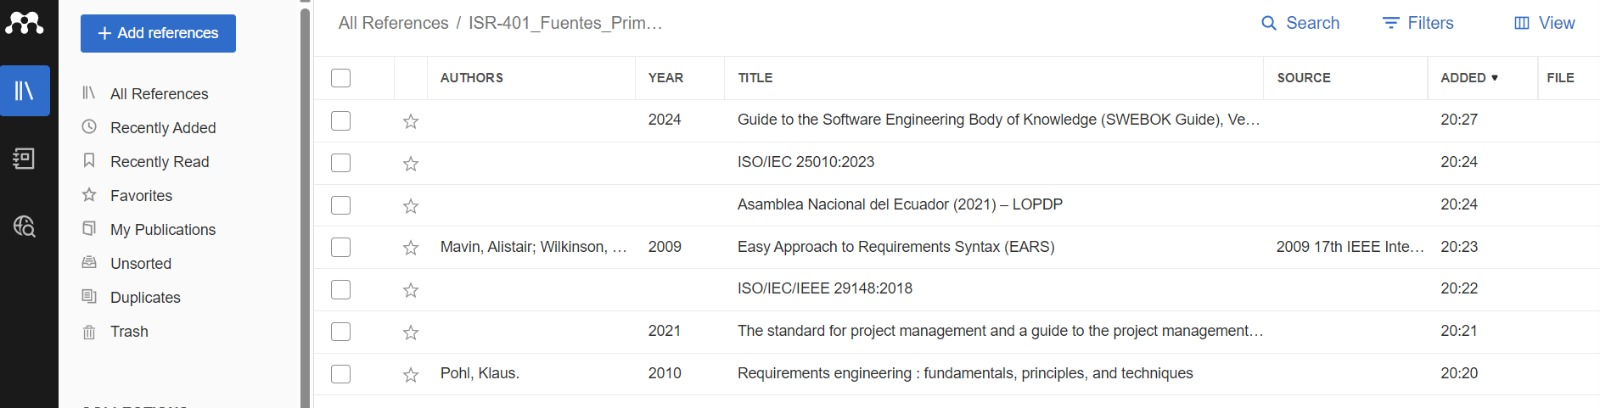
\includegraphics[width=4.95\linewidth, height=6.2cm, keepaspectratio]{Figuras/Evidencia_mendeley.jpeg}        
        }
    }
}\caption{}\label{Figuras/Evidencia_mendeley.jpeg}\end{figure}

\section{Anexo C. Guía de continuación técnica}
\begin{enumerate}
\item Revisar el código fuente para confirmar tecnología, persistencia, arquitectura e interfaces reales.
\item Aprobar la asignación de cinco funciones entre los tres estudiantes y documentar contribuciones individuales.
\item Verificar con el docente los títulos exactos de subtemas 2.1--2.6 y los cuatro temas que exige el mapa.
\item Reemplazar los perfiles ficticios por fuentes reales cuando existan interesados accesibles.
\item Comprobar los 20 requisitos en un entorno controlado con datos sintéticos y registrar resultados verdaderos.
\item Validar los cinco objetivos de calidad, en particular sus umbrales, antes de aprobar una línea base.
\item Registrar las referencias en Zotero o Mendeley y tomar la captura real de biblioteca para el anexo.
\item Publicar LaTeX, BibTeX, diagrama editable, capturas anonimizadas y PDF compilado en el repositorio personal correspondiente.
\end{enumerate}

\end{document}
